%%%%%%%%%%%%%%%%%%%%%%%%%%%%%%%%%%%%%%%%%%%%%%%%%%%%%%%%%%%%%%%
%
% F1000Research is an open access publishing platform, with rapid publication times and an open and transparent peer review process. This template is for Software Tool articles, which should include the rationale for the development of the tool and details of the code used for its construction. The article should provide examples of suitable input data sets and include an example of the output that can be expected from the tool and how this output should be interpreted.
%
%%%%%%%%%%%%%%%%%%%%%%%%%%%%%%%%%%%%%%%%%%%%%%%%%%%%%%%%%%%%%%%
%
% For more detailed article preparation guidelines, please see:
% https://f1000research.com/for-authors/article-guidelines/software-tool-articles
%
% For more information on the F1000Research publishing model please see:
% https://f1000research.com/about

\documentclass[10pt,a4paper]{article}
\usepackage{f1000_styles}
\usepackage{subcaption}

%% Default: numerical citations
% \usepackage[numbers]{natbib}

%% Uncomment this lines for superscript citations instead
% \usepackage[super]{natbib}

% Uncomment these lines for author-year citations instead
\usepackage[round]{natbib}
\let\cite\citep

\begin{document}
\pagestyle{fancy}

\title{High-dimensional regression and network learning with QIIME 2}
%\titlenote{Please provide a concise and specific title that clearly reflects the content of the article.}
\author[1,2]{Oleg Vlasovets}
\author[3]{Fabian Schaipp}
\author[4]{L\'eo Simpson}
\author[5]{Evan Bolyen}
\author[1,2,6]{Christian L. M\"uller}

\affil[1]{Computational Health Center, Helmholtz Munich}
\affil[2]{Ludwig-Maximilians-Universität M\"unchen, M\"unchen, Germany}
\affil[3]{Technical University M\"unchen, M\"unchen, Germany}
\affil[3]{Albert-Ludwigs-University Freiburg, Freiburg, Germany}
\affil[4]{Northern Arizona University, Flagstaff, USA}
\affil[5]{Center for Computational Mathematics, Flatiron Institute, New York, USA}

\maketitle
\thispagestyle{fancy}

% Please list all authors that played a significant role in developing the software tool and/or writing the article. Please provide full affiliation information (including full institutional address, ZIP code and e-mail address) for all authors, and identify who is/are the corresponding author(s).
\phantom{line keeping abstract on the left side}
\\
\\
\begin{abstract}

% Abstracts should be up to 300 words and provide a succinct summary of the article. Although the abstract should explain why the article might be interesting, care should be taken not to inappropriately over-emphasise the importance of the work described in the article. Citations should not be used in the abstract, and abbreviations, if needed, should be spelled out in full.


We introduce software for solving high-dimensional statistics problems in QIIME2 and illustrate several analysis use cases on soil microbiome data. Our software framework comprises two plugins, q2-classo and q2-gglasso, which 
enable sparse compositional regression and classification modeling and microbial network estimation, respectively. Both plugins are seamlessly integrated within the QIIME2 software ecosystem, one of the most popular open-source bioinformatic platforms for microbiome data analysis. Despite the comprehensive list of existing QIIME2 plugins for downstream analysis of microbiome data, our software includes several rigorous statistical estimators for microbiome data that have not yet made available in QIIME2, including estimators for sparse compositional regression and classification, sample covariance estimation, sparse inverse covariance estimation, and robust principal component analysis. All estimation procedures are accompanied by diagnostic plots and summary statistics as well as interactive visualizations, allowing the user to inspect and the resulting estimators.  
% \begin{minipage}{0.49\textwidth}
%     % Your content for the first minipage

% \end{minipage}
% \hfill
% \begin{minipage}{0.49\textwidth}
%     % Your content for the second minipage
%     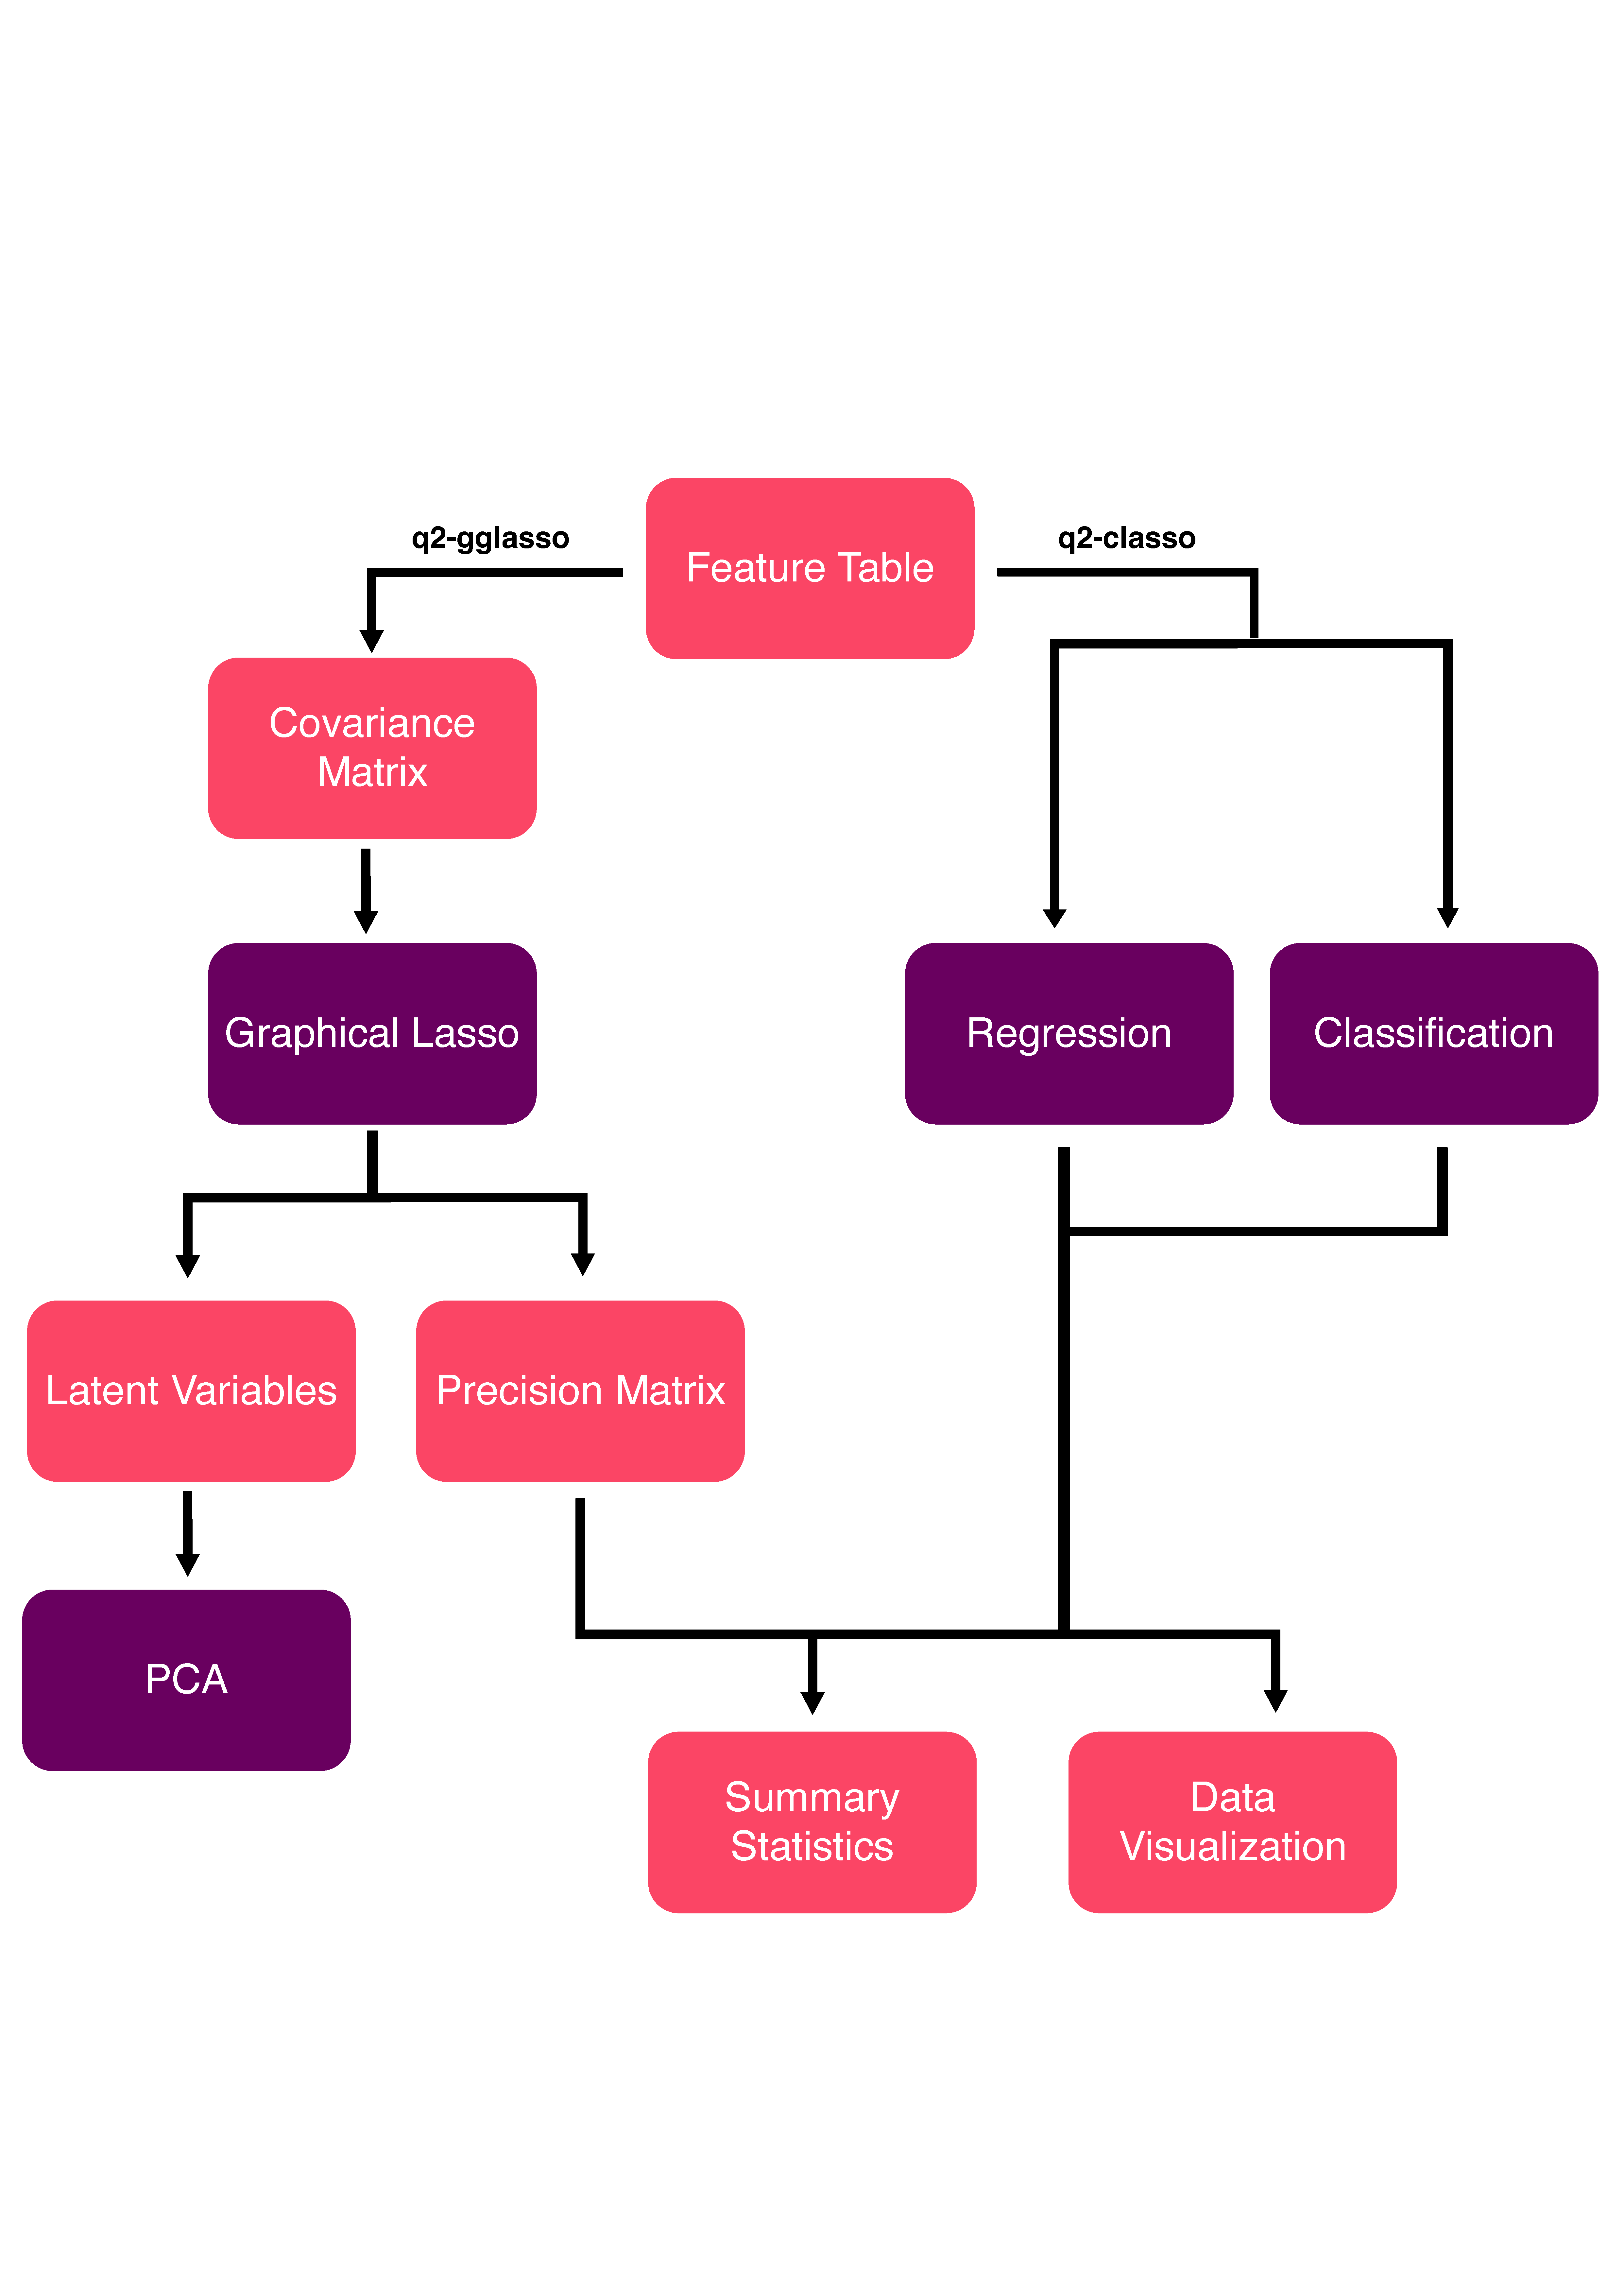
\includegraphics[width=\linewidth]{figures/q2/overview.pdf}
%     \caption{High-dimensional statistics with QIIME2.}
%     \label{fig:q2_overview}
% \end{minipage}



\end{abstract}
% \begin{document}
% \pagestyle{fancy}




% \maketitle
% \thispagestyle{fancy}

% % Please list all authors that played a significant role in developing the software tool and/or writing the article. Please provide full affiliation information (including full institutional address, ZIP code and e-mail address) for all authors, and identify who is/are the corresponding author(s).
% % \\
% % \\

% \begin{abstract}



% \end{abstract}

\section*{\color{f1ROrange}Keywords}

% Please list up to eight relevant keywords that describe the subject of their article. These will improve the visibility of your article.
QIIME2, compositional data, log-contrast regression, classification, graphical lasso, model selection

\clearpage
\pagestyle{fancy}
\section*{Introduction}

\begin{minipage}{0.5\textwidth}
    % Your content for the first minipage
    % Explain what QIIME2 is and what functionality related to statistics does it have.
    Microbiome data typically contains the large number of microbial features (also called "taxa") identified in high-throughput sequencing experiments. And high-dimensional statistics provides methods tailored to handle the intricacies of microbiome data. These methods assess microbial interactions, classify taxa, unveil patterns that may be indicative of biological phenomena, such as shifts in community composition or associations with specific environmental factors.

    Several software tools are available for the analysis of microbiome data, including MicrobiomeAnalyst \cite{dhariwal2017microbiomeanalyst}, Qiita \cite{gonzalez2018qiita}, STAMP \cite{parks2014stamp}, and mothur \cite{schloss2009introducing}. However, some of these tools are designed for specific tasks, e.g., USEARCH \cite{edgar2010search}, while others may require extensive knowledge of programming or lack examples and user support.
    
    QIIME2 is open-source bioinformatics software platform designed for the analysis of microbiome data. It strikes a balance between user programming expertise, the breadth of functionality, and a substantial user base with active support from developers and users on the community forum.
    
\end{minipage}
\hfill
\begin{minipage}{0.49\textwidth}
    % Your content for the second minipage
        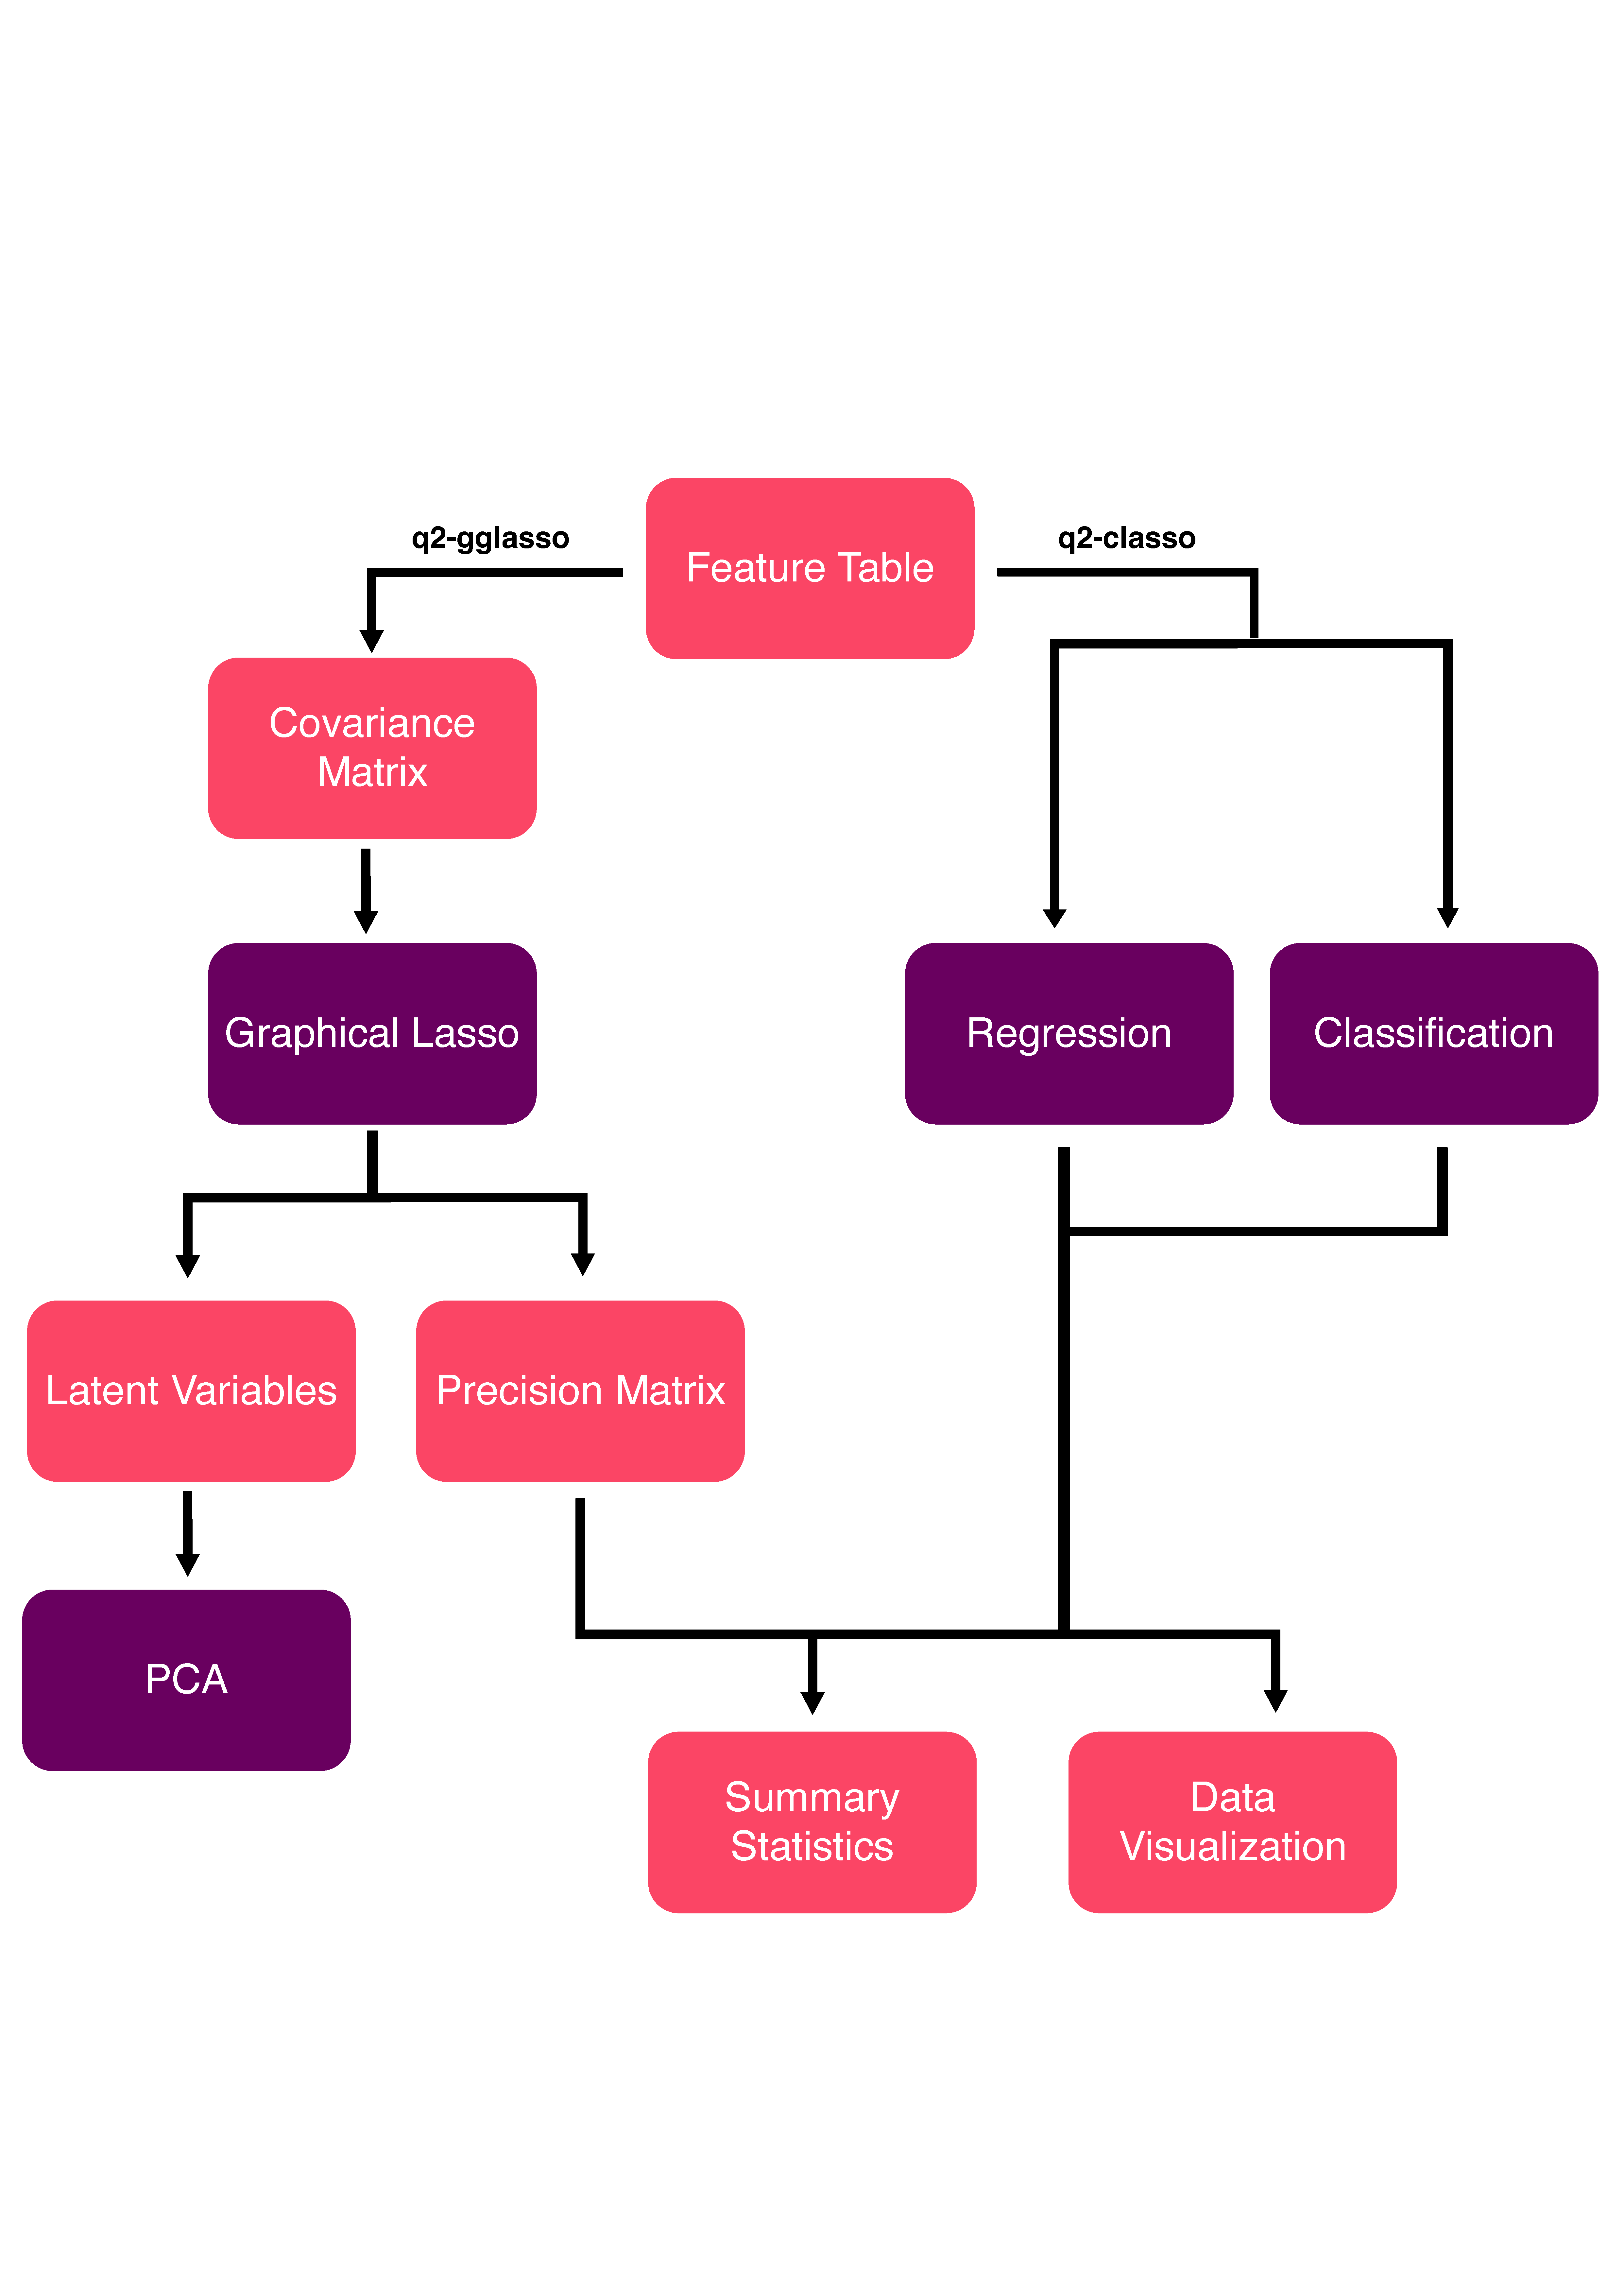
\includegraphics[width=0.9\linewidth]{figures/q2/overview.pdf}
        \captionof{figure}{High-dimensional statistics with QIIME2.}
        \label{fig:q2_overview}
\end{minipage}

 \par QIIME2 has a collection of plugins specifically developed to preprocess raw sequences from high-throughput sequencing datasets, preparing them for downstream analyses. For the actual analysis, it includes plugins that facilitate the investigation of microbial diversity, community structure, differential abundance testing, and more \cite{bolyen2019reproducible}. 

\par Within classification and regression tasks, \cite{bokulich2018q2} provide a set of standard machine learning models implemented in q2-sample-classifier plugin. These models include Ridge \cite{hoerl1970ridge}, and Lasso \cite{tibshirani1996regression} regression, along with kNN classifiier \cite{altman1992introduction} and tree-based classification algorithms \cite{breiman2001random}. In addition, there are various feature selection techniques from scikit-learn \cite{pedregosa2011scikit}, such as recursive feature elimination with cross-validation (RFECV) and randomized search cross-validation. 

\par For a differential abundance analysis, there are plugins that are aware of data compositionality \cite{aitchison1982statistical} mirroring popular frameworks such as ANCOM-BC \cite{lin2020analysis}, Songbird \cite{morton2019establishing} and Gneiss \cite{morton2017balance} where various data transformations, such as the isometric log-ratio (ILR) are implemented.

\par QIIME2 also provides plugins for statistical analysis of biological networks. For instance, SCNIC \cite{shaffer2023scnic} simplifies the creation of correlation networks from feature tables, offering flexibility in selecting metrics for network generation. Also, q2-makarsa incorporates some functionality including sparse graphical models and model selection from a popular SpiecEasi framework \cite{kurtz2015sparse}. DEICODE \cite{martino2019novel} facilitates Principal Component Analysis (PCA) where zero values have minimal impact on the resulting ordination. In addition, the principal components can be visualized with Emperor plugin introduced by \cite{vazquez2017bringing}.


Nevertheless, to conduct advanced statistical analyses on biological samples users often lack "out of the box" options. Consequently, they have to export the data and explore alternative solutions, such as R or Python libraries, where the required functionality exists. The pipeline depicted in   \autoref{fig:q2_overview} outlines the functionality implemented in two QIIME2 plugins namely q2-classo for regression and classification tasks, and q2-gglasso for network learning. Together, these plugins address gaps in the existing functionality within QIIME2, offering comprehensive documentation with tutorials on applying such models in different scenarios and featuring interactive visualizations ready for use in publications.


% The introduction provides context as to why the software tool was developed and what need it addresses.  It is good scholarly practice to mention previously developed tools that address similar needs, and why the current tool is needed. 


\section*{Methods}
% \subsection*{Implementation}

% For software tool papers, this section should address how the tool works and any relevant technical details required for implementation of the tool by other developers.

Our software provides sparse and robust linear regression and classification models with linear equality constraints \cite{Simpson2021}. It also provides solvers for general graphical problems \cite{Schaipp2021}. In the following, we describe the underlying statistical models and highlight essential features of our software, including model selection.

\subsection*{Regression/Classification}

% This part of the methods should include the minimal system requirements needed to run the software and an overview of the workflow for the tool for users of the tool.

% add figure with X and Y blocks 

We consider the following statistical forward model:

\begin{equation}
    Y = X\beta + \sigma \epsilon \qquad \textrm{subject to} \quad C \beta = 0.
\end{equation}

where $X \in \mathbb{R}^{n \times p}$ is a given data matrix, and the vector $y \in \mathbb{R}^n$ is a continuous or binary response vector, matrix $C$ represents a general constraint matrix. The vector $\beta \in \mathbb{R}^p$ contains the unknown coefficients, $\sigma$ represents an unknown scale, and $\epsilon \in \mathbb{R}^n$ is a noise vector. To infer unknown coefficients and scale, we solve optimization problem in the form:

\begin{equation}
    \begin{aligned}\label{eq:r1}
     \min _{\beta \in \mathbb{R}^p, \sigma \in \mathbb{R}_0} f(X \beta-y, \sigma)+\lambda\|\beta\|_1 \quad \text { subject to } \quad C \beta=0
    \end{aligned}
\end{equation}

for several convex loss functions $f(\cdot, \cdot)$. This includes the constrained Lasso, the constrained scaled Lasso, and sparse Huber M-estimators with linear equality constraints \cite{combettes2020perspective}.

%%% Standard R1
% \begin{equation}
%     \begin{aligned}\label{eq:r1}
%     \min_{\beta \in \mathbb{R}^d} \left\lVert X\beta - y \right\rVert^2 + \lambda \left\lVert \beta\right\rVert_1 \qquad \textrm{subject to:} \quad C \beta=0
%     \end{aligned}
% \end{equation}

% \subsection*{Classification}


Notable use cases include (sparse) log-contrast regression with compositional data $X$, which necessitates the constraint $1^T_p \beta = 0$ \cite{aitchison1984log}. We implement a log-contrast model as outlined by \cite{combettes2020perspective} and its extension of a tree-aggregated model, as proposed by \cite{bien2021tree}, expressed as follows:

\begin{equation}\label{eq:slc}
    \begin{aligned}
        \min_{\beta \in \mathbb{R}^p} f(y - \log(X) \beta) + \lambda P (\beta)\quad \text{subject to} \quad 1_p^T \beta = 0
    \end{aligned}
\end{equation}


where a logarithmic transformation of $X$ converts taxa differences into log-ratios. Tree-aggregated model estimates a convex penalty \(P(\beta)\) specifically designed to encourage the structure of \(\beta\) based on subtrees within a taxonomic tree.

% \subsection*{Tree-aggregated model}


\subsection*{Model selection}
In our framework, several model and feature selection procedures are available for regression and classification tasks:

\begin{itemize}
    \item \textbf{Cross-validation:} the regularization parameter $\lambda$ is chosen through k-fold cross-validation, considering $\lambda$ within the interval $[\lambda_{\text{min}}, \lambda_{\text{max}}]$. Both the Minimum Mean Squared Error (MSE) and the "One-Standard-Error rule" (1SE) criteria, as discussed by \cite{hastie2009elements}, are applicable.
    
    \item \textbf{Stability selection:} the regularization parameter $\lambda$ is facilitated through stability selection \cite{combettes2020perspective}.
    Three distinct modes are available: selection at a predetermined $\lambda$, the selection of the first $q$ variables entering the path (default setting), and the selection of the $q$ largest coefficients (in absolute value) across the path \cite{meinshausen2010stability}.
    
    \item \textbf{Stability selection }+ \textbf{theoretical lambda $\lambda_{0}$}: this approach is similar to the stability selection approach. However, \cite{combettes2020perspective} propose to select nonzero coefficients for every subsample at the regularization parameter $\lambda_{0}$ as introduced by \cite{shi2016regression}. Notably, the value of $\lambda_{0}$ depends on the sample size and therefore requires adaptation to the specific dataset.

\end{itemize}





% \begin{itemize}
%     \item CV
%     \item stability selection
%     \item theoretical lambda

% Just say that these methods are supported and give links to the corresponding papers.
% \end{itemize}


\subsection*{Network learning}
The unit-sum constraint in Eq. \autoref{eq:slc} is one of the difficulties encountered when dealing with compositional data.  In the context of correlation estimation, a widely adopted strategy \cite{kurtz2015sparse} is to apply the centered log-ratio transform (clr) \cite{aitchison1982statistical} to the compositional vector of each sample $x_i \in \mathbb{S}^p$. We implement both the clr-transform and a modified version proposed by \cite{yoon2019microbial}, where the geometric mean $\widetilde{g}$ is calculated for the non-zero elements of \(x_i\), avoiding the need for adding a pseudo count:

\begin{equation}
    \begin{gathered}
        \mathbf{z}_i = \operatorname{mclr}_{\varepsilon}(\mathbf{x}_i)
        = \left[0, \ldots, 0, \log\left\{x_{i(q+1)} / \widetilde{g}(\mathbf{x}_i)\right\}+\varepsilon, \ldots, \log\left\{x_{i p} / \widetilde{g}(\mathbf{x}_i)\right\}+\varepsilon\right] \\
        \widetilde{g}(\mathbf{x}_i) = \left(\prod_{j=q+1}^p x_{i j}\right)^{1/(p-q)}
    \end{gathered}
\end{equation}

The covariance matrix \(S\) describes associations in bacterial networks, and it can be derived from the transformed vectors \(\mathbf{z}_i\), where \(i = 1, \ldots, n\), rather than directly from the original compositions \(\mathbf{X}\). The inverse covariance matrix \(\Sigma^{-1}\) characterizes the conditional independence among the vectors \(\mathbf{z}_i\). Although \(S^{-1}\), if it exists, serves as the maximum-likelihood estimator of the inverse covariance, it is not guaranteed to be sparse which is another pivotal characteristic of microbial data. Hence, we solve the nonsmooth convex optimization problem, known as the Graphical Lasso, in a form:

\begin{equation}
    \begin{gathered}
        \min_{\Theta \in \mathbb{S}^p_{++}}:-\log (\operatorname{det}|\Theta|)+\langle S, \Theta\rangle+\lambda\|\Theta\|_{1, \text{od}}
    \end{gathered}
\end{equation}
This formulation requires both conditional independence and sparsity. Here, \(\mathbb{S}^p_{++}\) represents symmetric positive definite  \(p \times p\) matrices, \(\|\cdot\|_1\) is the sum of absolute values of all off-diagonal elements, and \(\operatorname{\langle \cdot, \cdot \rangle}\) denotes the trace of a matrix.



% Consider a multivariate Gaussian variable:

% \begin{equation}
%     \begin{gathered}
%         X \sim N (\mu, \Sigma) \in \mathbb{R}^p \\
%     \end{gathered}
% \end{equation}





% \begin{itemize}
%     \item mclr transformation and Spring paper (from X to Z)
%     \item adaptive graphical lasso
%     \item graphical lasso with a low-rank (Z - data, Y - covariates)
% \end{itemize}

% \begin{equation}
%     \begin{aligned}\label{eq:c1}
%     \min _{\beta \in \mathbb{R}^d} \max \left(0,1-y^t X \beta\right)^2+\lambda\|\beta\|_1 \qquad \textrm{subject to:} \quad C \beta=0
%     \end{aligned}
% \end{equation}


% \section*{Results} % Optional - only if novel data or analyses are included
% This section is only required if the paper includes novel data or analyses, and should be written as a traditional results section.

\newpage
\section*{Use Cases} % Optional - only if no new datasets are included
% This section is required if the paper does not include novel data or analyses. 
% Examples of input and output files should be provided with some explanatory context.  Any novel or complex variable parameters should also be explained in sufficient detail to allow users to understand and use the tool's functionality. \textbf{Data input for use cases must be provided}

In our example, we showcase the application of our QIIME2 plugins for high-dimensional statistics using the Atacama soil microbiome dataset \cite{neilson2017significant}. With q2-gglasso we solve various graphical lasso problems to identify microbial associations which we later assess by fitting sparse log-contrast models implemented in q2-classo. Microbiome bioinformatics analyses was conducted using QIIME 2 version 2022.4 \cite{bolyen2019reproducible}. The processing of raw sequence data involved demultiplexing and quality filtering, facilitated by the q2‐demux plugin. Subsequent denoising was performed using DADA2 \cite{callahan2016dada2} through the q2‐dada2 plugin. Taxonomic assignments for Amplicon Sequence Variants (ASVs) were accomplished using the q2‐feature‐classifier \cite{bokulich2018optimizing} with the naive Bayes taxonomy classifier, trained on the Silva Database \cite{quast2012silva}.

\subsection*{Data transformation}
Microbiome data typically represents the relative abundances of different microbial taxa within a sample. However, these relative abundances are constrained because the total sum of relative abundances adds up to a constant \cite{gloor2017microbiome}. This compositional constraint can cause statistical issues and distort the interpretation of the data. To address these limitations, we apply the mclr-transformation (  \autoref{fig:acm_data}) which converts the compositional data into an unconstrained data space \cite{yoon2019microbial}. After the pre-processing, our data consists of $13$ distinct microbial taxa and $50$ individual samples (\autoref{tab:org_acm}). In addition, we select covariates related to the soil microbiome data, including pH, elevation (m), average soil temperature (t°), and humidity (\%). The covariates live on a different scale, so we perform a standard scaling procedure from \href{https://scikit-learn.org/stable/modules/generated/sklearn.preprocessing.StandardScaler.html}{scikit-learn} \cite{scikit-learn}, where the data is also centered before scaling to unit standard deviation (\autoref{fig:acm_covariates}). 

% \begin{verbatim}

% qiime gglasso transform-features \
%      --p-transformation mclr \
%      --p-add-metadata False \
%      --p-scale-metadata False \
%      --i-table data/pandas-counts.qza \
%      --i-taxonomy data/classification.qza \
%      --m-sample-metadata-file data/selected-atacama-sample-metadata.tsv \
%      --o-transformed-table data/atacama-table-mclr.qza \
%      --verbose
% \end{verbatim}

\begin{figure}[h]
    \centering
    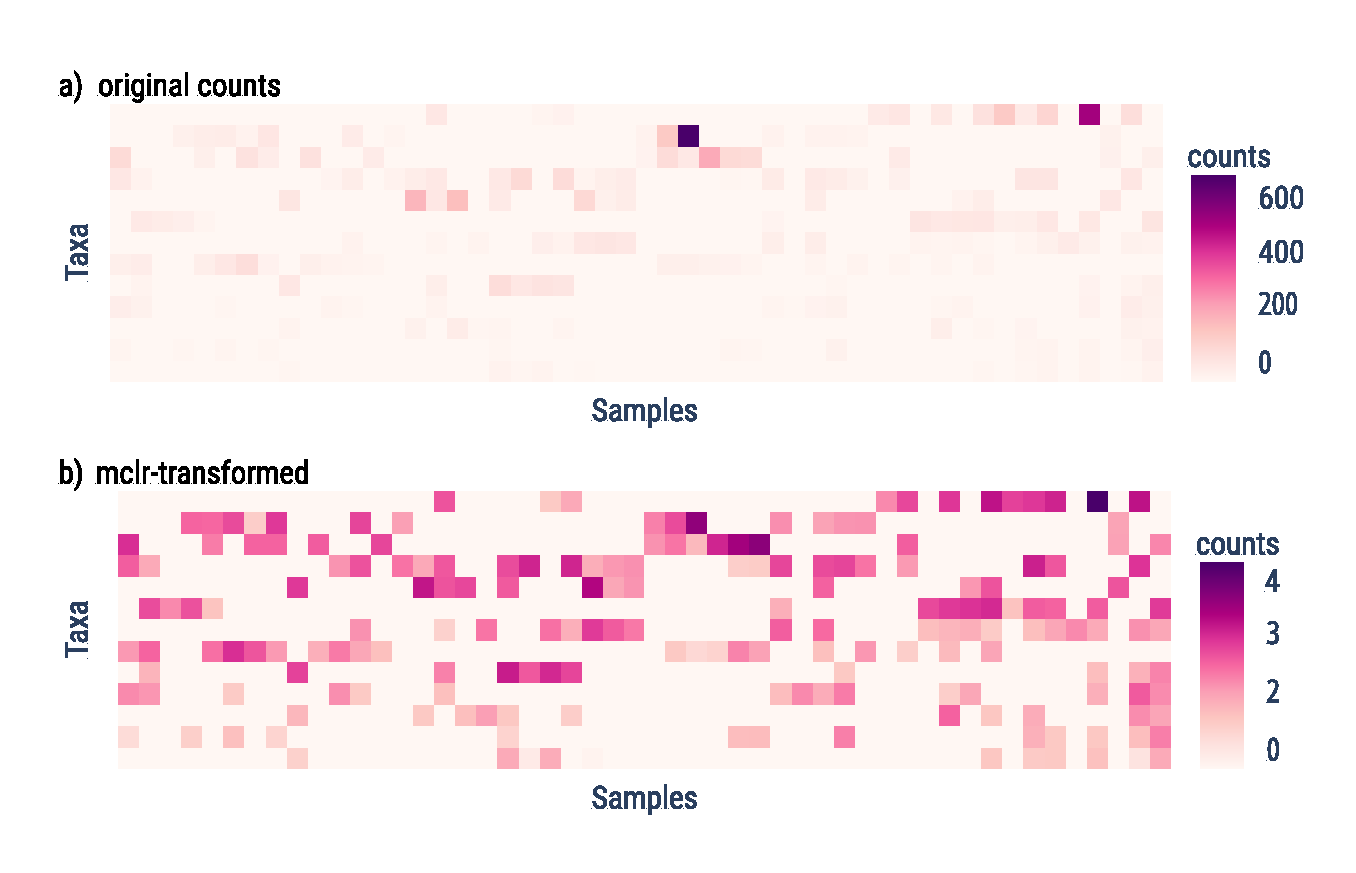
\includegraphics[width=0.65\linewidth]{figures/q2/acm_data.pdf}
    \caption{Atacama soil microbiome a) before and b) after mclr-transformation.}
    \label{fig:acm_data}
\end{figure}


\subsection*{General Graphical Lasso models}
\par We start our analysis by looking at the empirical correlation matrix $\hat{S_{0}}$ and corresponding network. In   \autoref{fig:gg_example}a, we observe two edges $e_{1} = (ASV_{6}, ASV_{11})$ and $e_{2} = (ASV_{1}, ASV_{5})$. Also, we see associations between $ASV_{1}$, $ASV_{5}$, $ASV_{6}$ and $ASV_{11}$ making this sub-graph fully connected. Under the sparsity assumption, we proceed to solve a single graphical lasso problem \cite{friedman2008sparse}. In   \autoref{fig:gg_example}b, we observe the persistence of the positive edges $e_{1}$ and $e_{2}$, and the sparse model has eliminated the rest of the edges. It is well-known that taxa correlate with specific environmental factors, such as pH, soil temperature, humidity, and elevation. We estimate the partial correlation between taxa and these covariates jointly by applying penalization procedure element-wise which is referred to as an adaptive graphical lasso solution $\hat\Theta_{Adapt}$. In   \autoref{fig:gg_example}c, we see the remaining positive edge $e_{2}$, and the previously identified edge $e_{1}$ can be attributed to the temperature since $ASV_{6}$ and $ASV_{11}$ no longer correlate with each other.

\begin{figure}[!h]
    \centering
    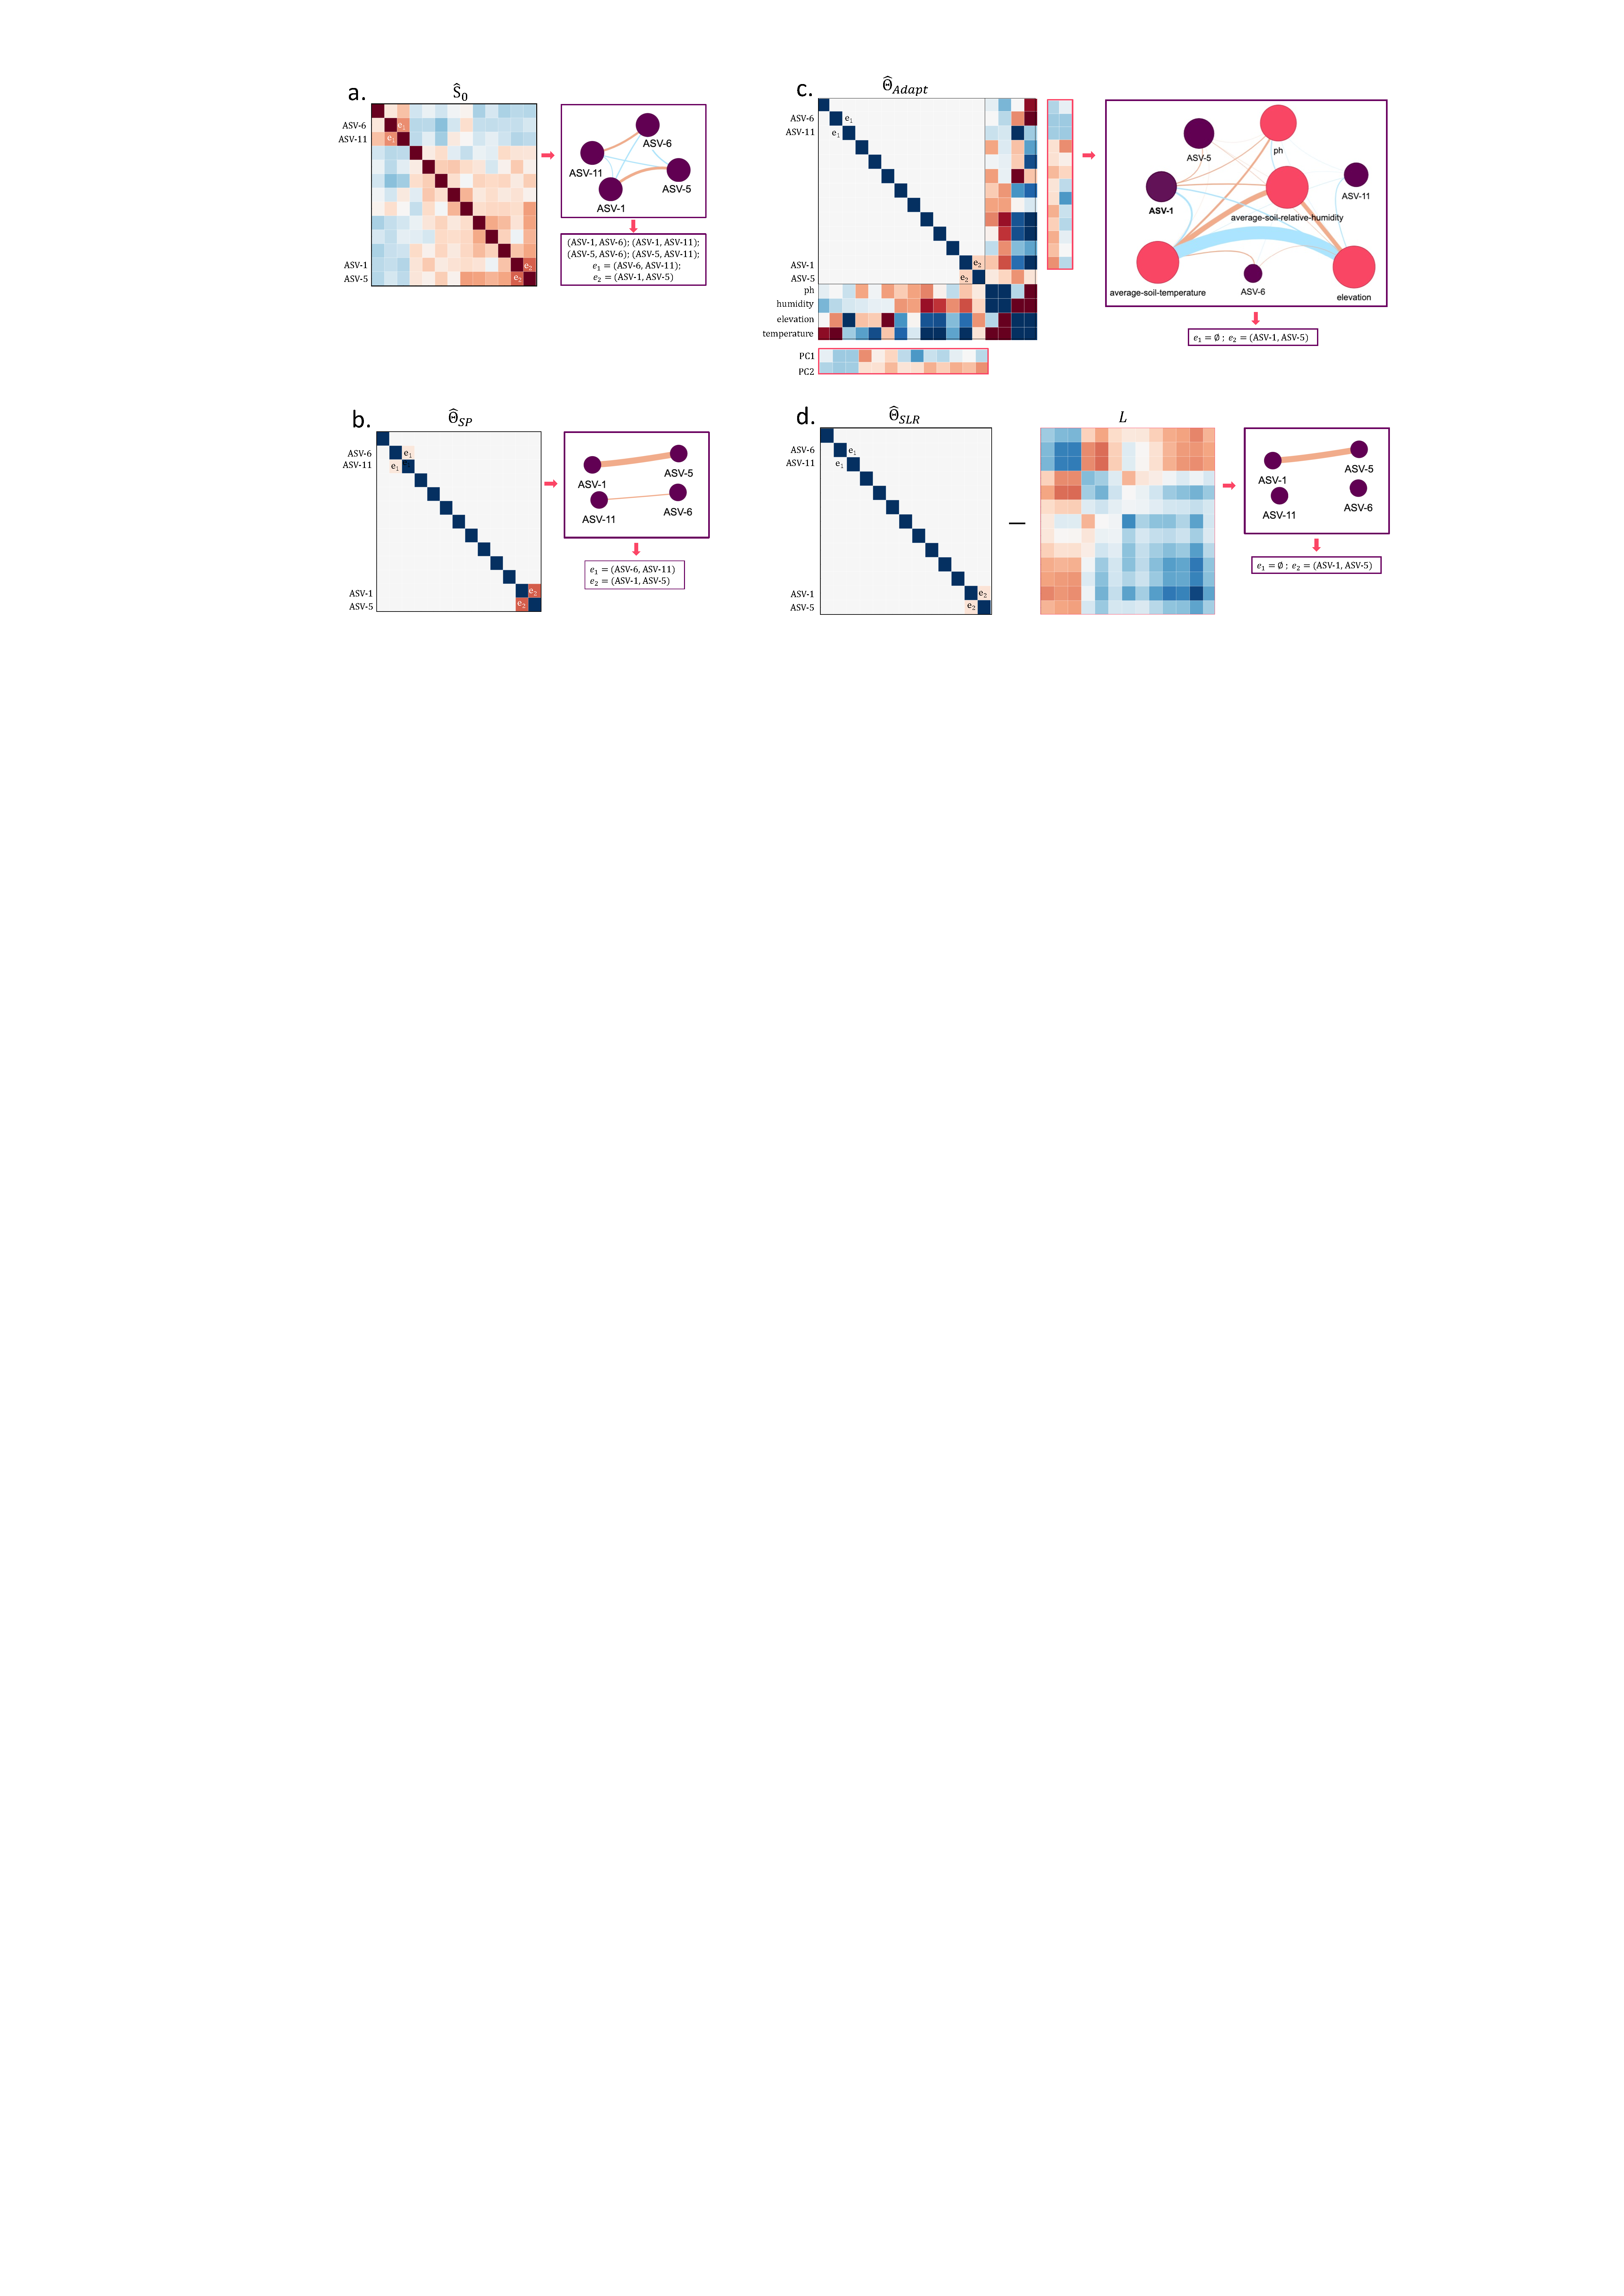
\includegraphics[width=\linewidth]{figures/q2/example_gglasso.pdf}
    \caption{General Graphical Lasso: a) empirical correlation; 
    b) sparse; c) adaptive d) sparse + low-rank models.}
    \label{fig:gg_example}
\end{figure}

\par In scenarios where covariates are missing or corrupted, it becomes challenging to capture the effects of hidden confounders. To address this issue, we solve a single graphical lasso with latent variables, i.e., sparse + low-rank model \cite{chandrasekaran2010latent}.   \autoref{fig:gg_example}d shows solution $\hat\Theta_{SLR}$ where $e_{2}$ remains, but $e_{1}$ disappears due to the low-rank component $L$. The network of $\hat\Theta_{SLR}$ is more similar to $\hat\Theta_{Adapt}$, which incorporates the available covariate information. We compare the first two principal components (PCs) of $L$ and compare them with the estimated covariates from the adaptive model. Notably, $PC_{1}$ captures the effect of pH, while $PC_{2}$ captures the effect of the average soil temperature.

\subsection*{Graphical Lasso with latent variables}
\par In a related study \cite{kurtz2019disentangling}, an alternative approach utilizing the sparse + low-rank model was explored. The authors used the low-rank part of the model to perform a robust principal component analysis (PCA) \cite{candes2011robust} of the microbial counts. In their analysis, they discovered that some correlations could be attributed to latent factors such as zero counts, compositional artifacts, and batch effects. In \autoref{fig:slr_example}, we replicate their example using the Atacama soil microbiome dataset. We assume that the top-left block of the empirical correlation matrix $\hat{S_{0}}$ is driven by a latent factor which is not taken into account. In the sparse solution $\hat\Theta_{SP}$, most of those spurious correlations are eliminated, but edge $e_{1}$ is still present and claims the direct association between two taxa. In contrast, the top-left block of $\hat\Theta_{SLR}$ does not exhibit any direct associations, as the low-rank component $L$ effectively captures the influence of latent confounders. This can be verified by projecting each sample from $Z_{mclr}$ onto the principal components of $L$ and examining the correlation between these PCs and the covariates. \autoref{fig:scatter_pc} shows the correlation between $PC_{1}$ and the average soil temperature and elevation. We observe that microbial compositions increase as the temperature rises, while they decline with an increase in elevation.

\begin{figure}[h]
    \centering
    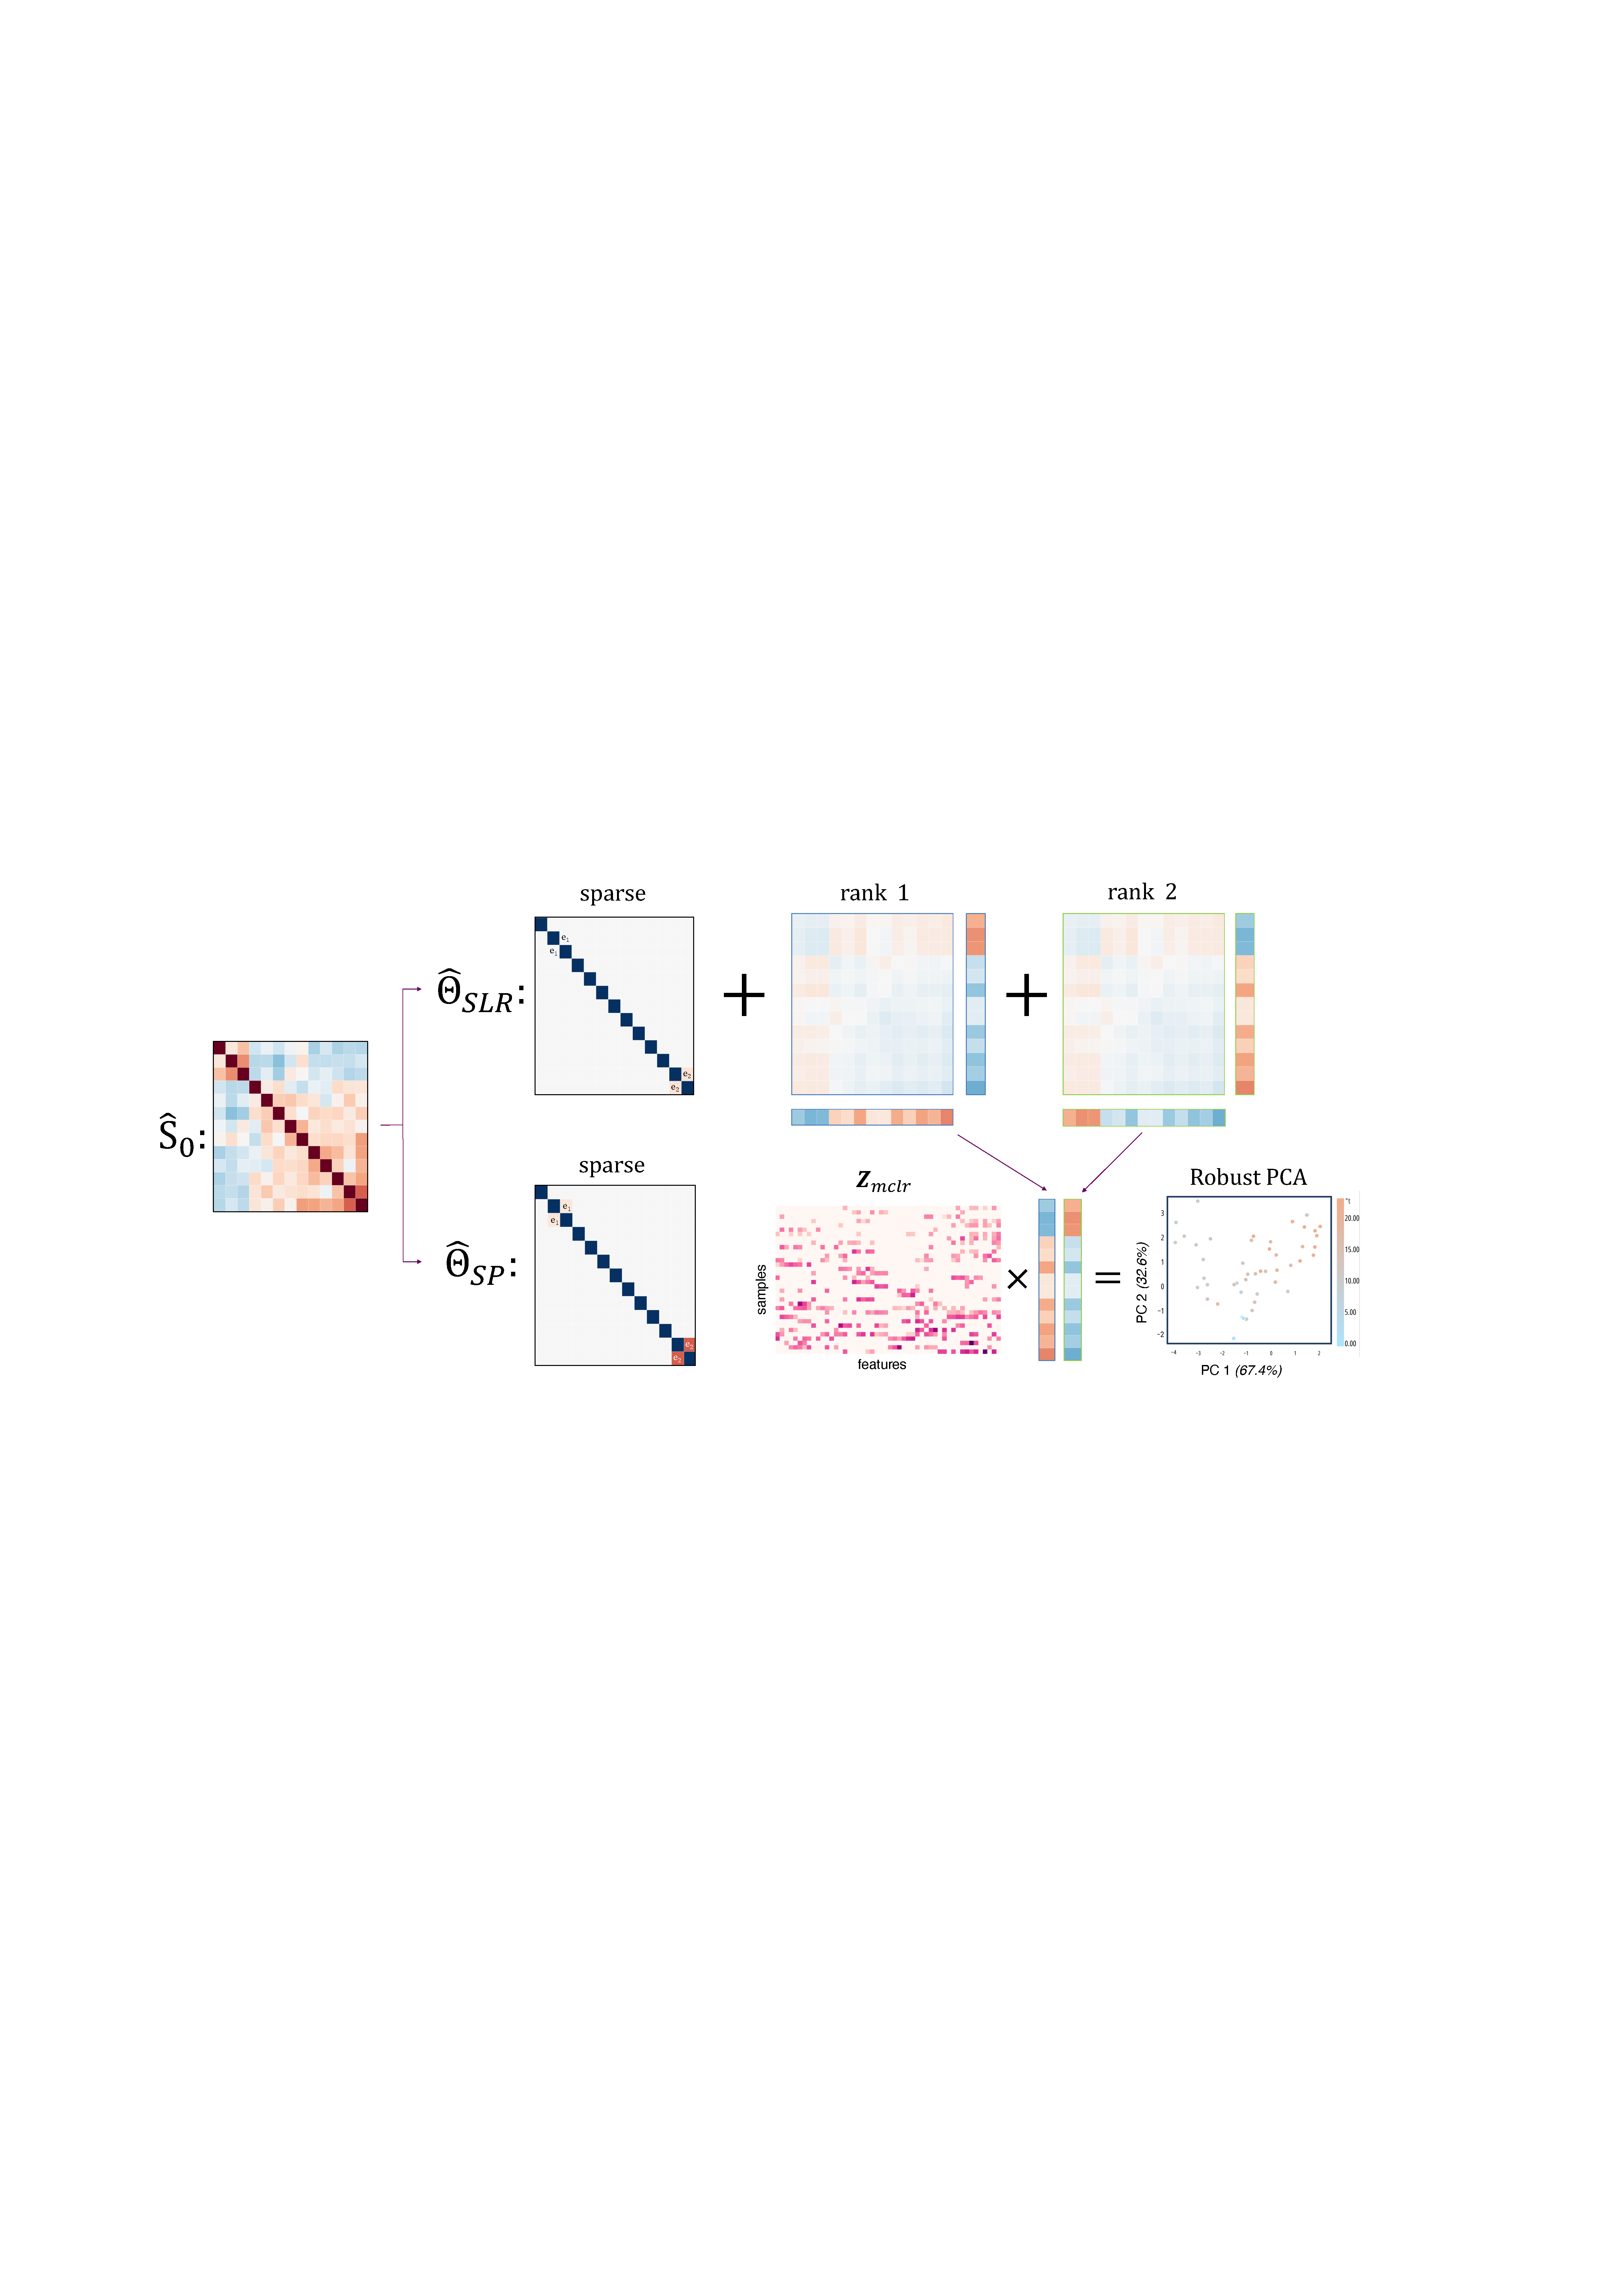
\includegraphics[width=0.85\linewidth]{figures/q2/slr_example.pdf}
    \caption{Example of using sparse + low-rank model for robust PCA.}
    \label{fig:slr_example}
\end{figure}

\begin{figure}[h]
    \centering
    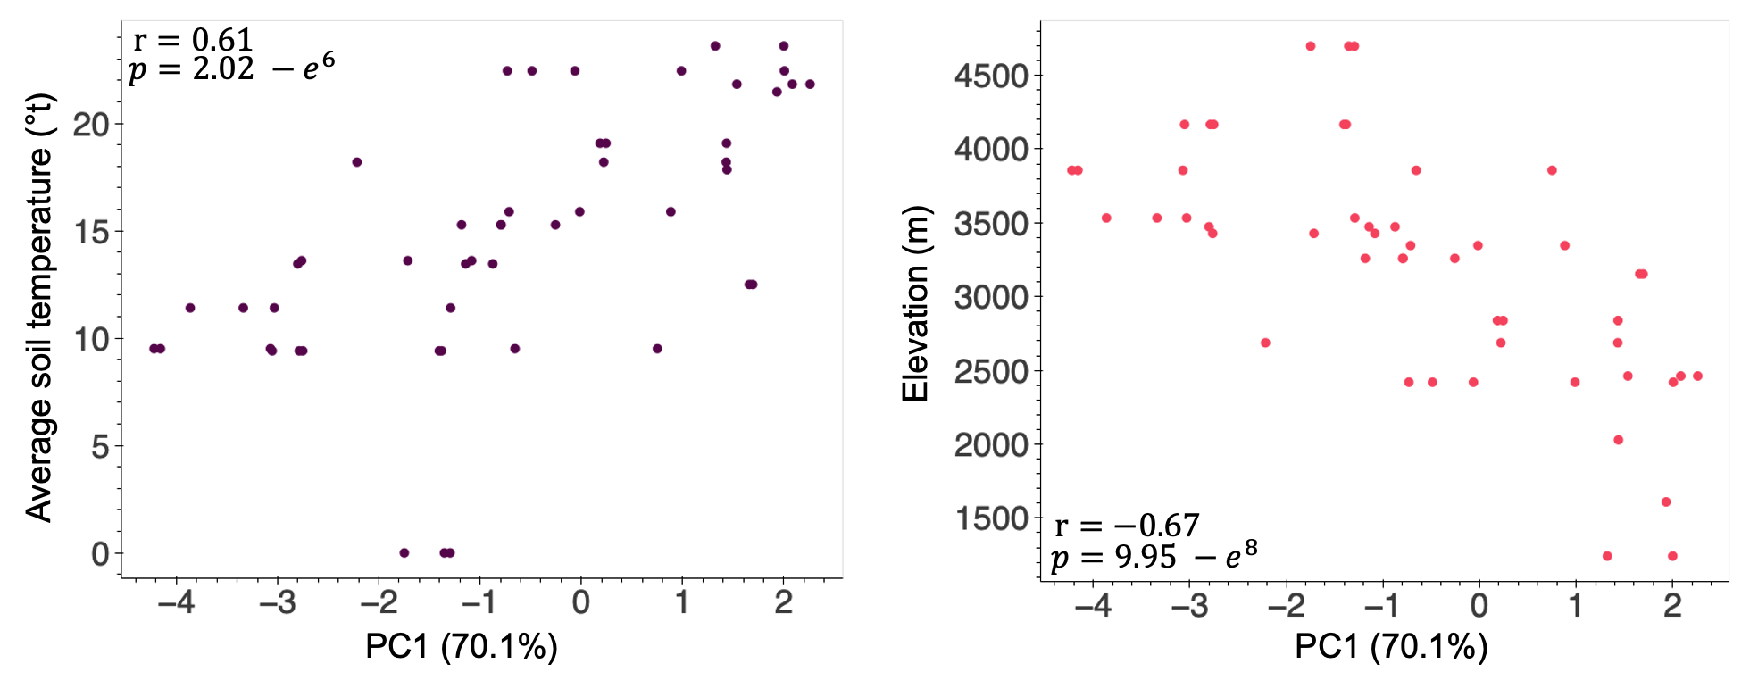
\includegraphics[width=0.8\linewidth]{figures/q2/scatter_pc.pdf}
    \caption{Relationship between PC1 and the average soil temperature (left), elevation (right).}
    \label{fig:scatter_pc}
\end{figure}

% \par To sum up, we present three distinct scenarios for using q2-gglasso, namely sparse, adaptive, and sparse + low-rank models. The results showcased that the sparse + low-rank model was able to effectively replicate a widely acknowledged biological phenomenon: the dependence of microbial compositions on environmental factors such as temperature and elevation. In line with the assumptions outlined in \cite{chandrasekaran2010latent}, we propose a framework which captures the underlying structure and interactions within the microbial community while promoting sparsity in the estimated network.

\newpage

\subsection*{Sparse log-contrast models}



\par Extending our previous analysis of the Atacama soil microbiome, now our objective is to predict the average soil temperature based on microbiome compositions and additional covariates. We address the problem outlined in \autoref{fig:slc}, which entails a linear model. Notably, this model incorporates an extra $1^T_p \beta = 0$ constraint on coefficients ($\beta$) to adjust for the compositionality. \autoref{fig:acm_reg} shows the solution ($R^2=0.707$) at the chosen parameter $\lambda=0.035$. The framework facilitates a stability selection procedure with a threshold probability ($P=0.7$) corresponding to the likelihood that $ASV_{4-9}$, $ASV_{11}$ and $ASV_{12}$ have been consistently chosen throughout the model selection process. It is noteworthy that $ASV_{7}$ and $ASV_{12}$ are the most predictive log-ratios, and concurrently, these same ASVs demonstrate the highest correlation with pH and average soil temperature (\autoref{fig:gg_example}). These covariates showed a significant impact on microbial compositions in the earlier network analysis.

% \begin{align*}
%     Y &= 0.467 + 0.304\cdot\textbf{ASV-2} - 0.197\cdot\textbf{ASV-4} - 0.086\cdot\textbf{ASV-6} + 0.378\cdot\textbf{ASV-7} \\
%     &\quad - 0.161\cdot\textbf{ASV-8} + 0.091\cdot\textbf{ASV-9} + 0.007\cdot\textbf{ASV-10} - 0.124\cdot\textbf{ASV-11} - 0.237\cdot\textbf{ASV-12} + 0.027\cdot\textbf{ASV-13}
% \end{align*}


\begin{figure}[!h]
    \centering
    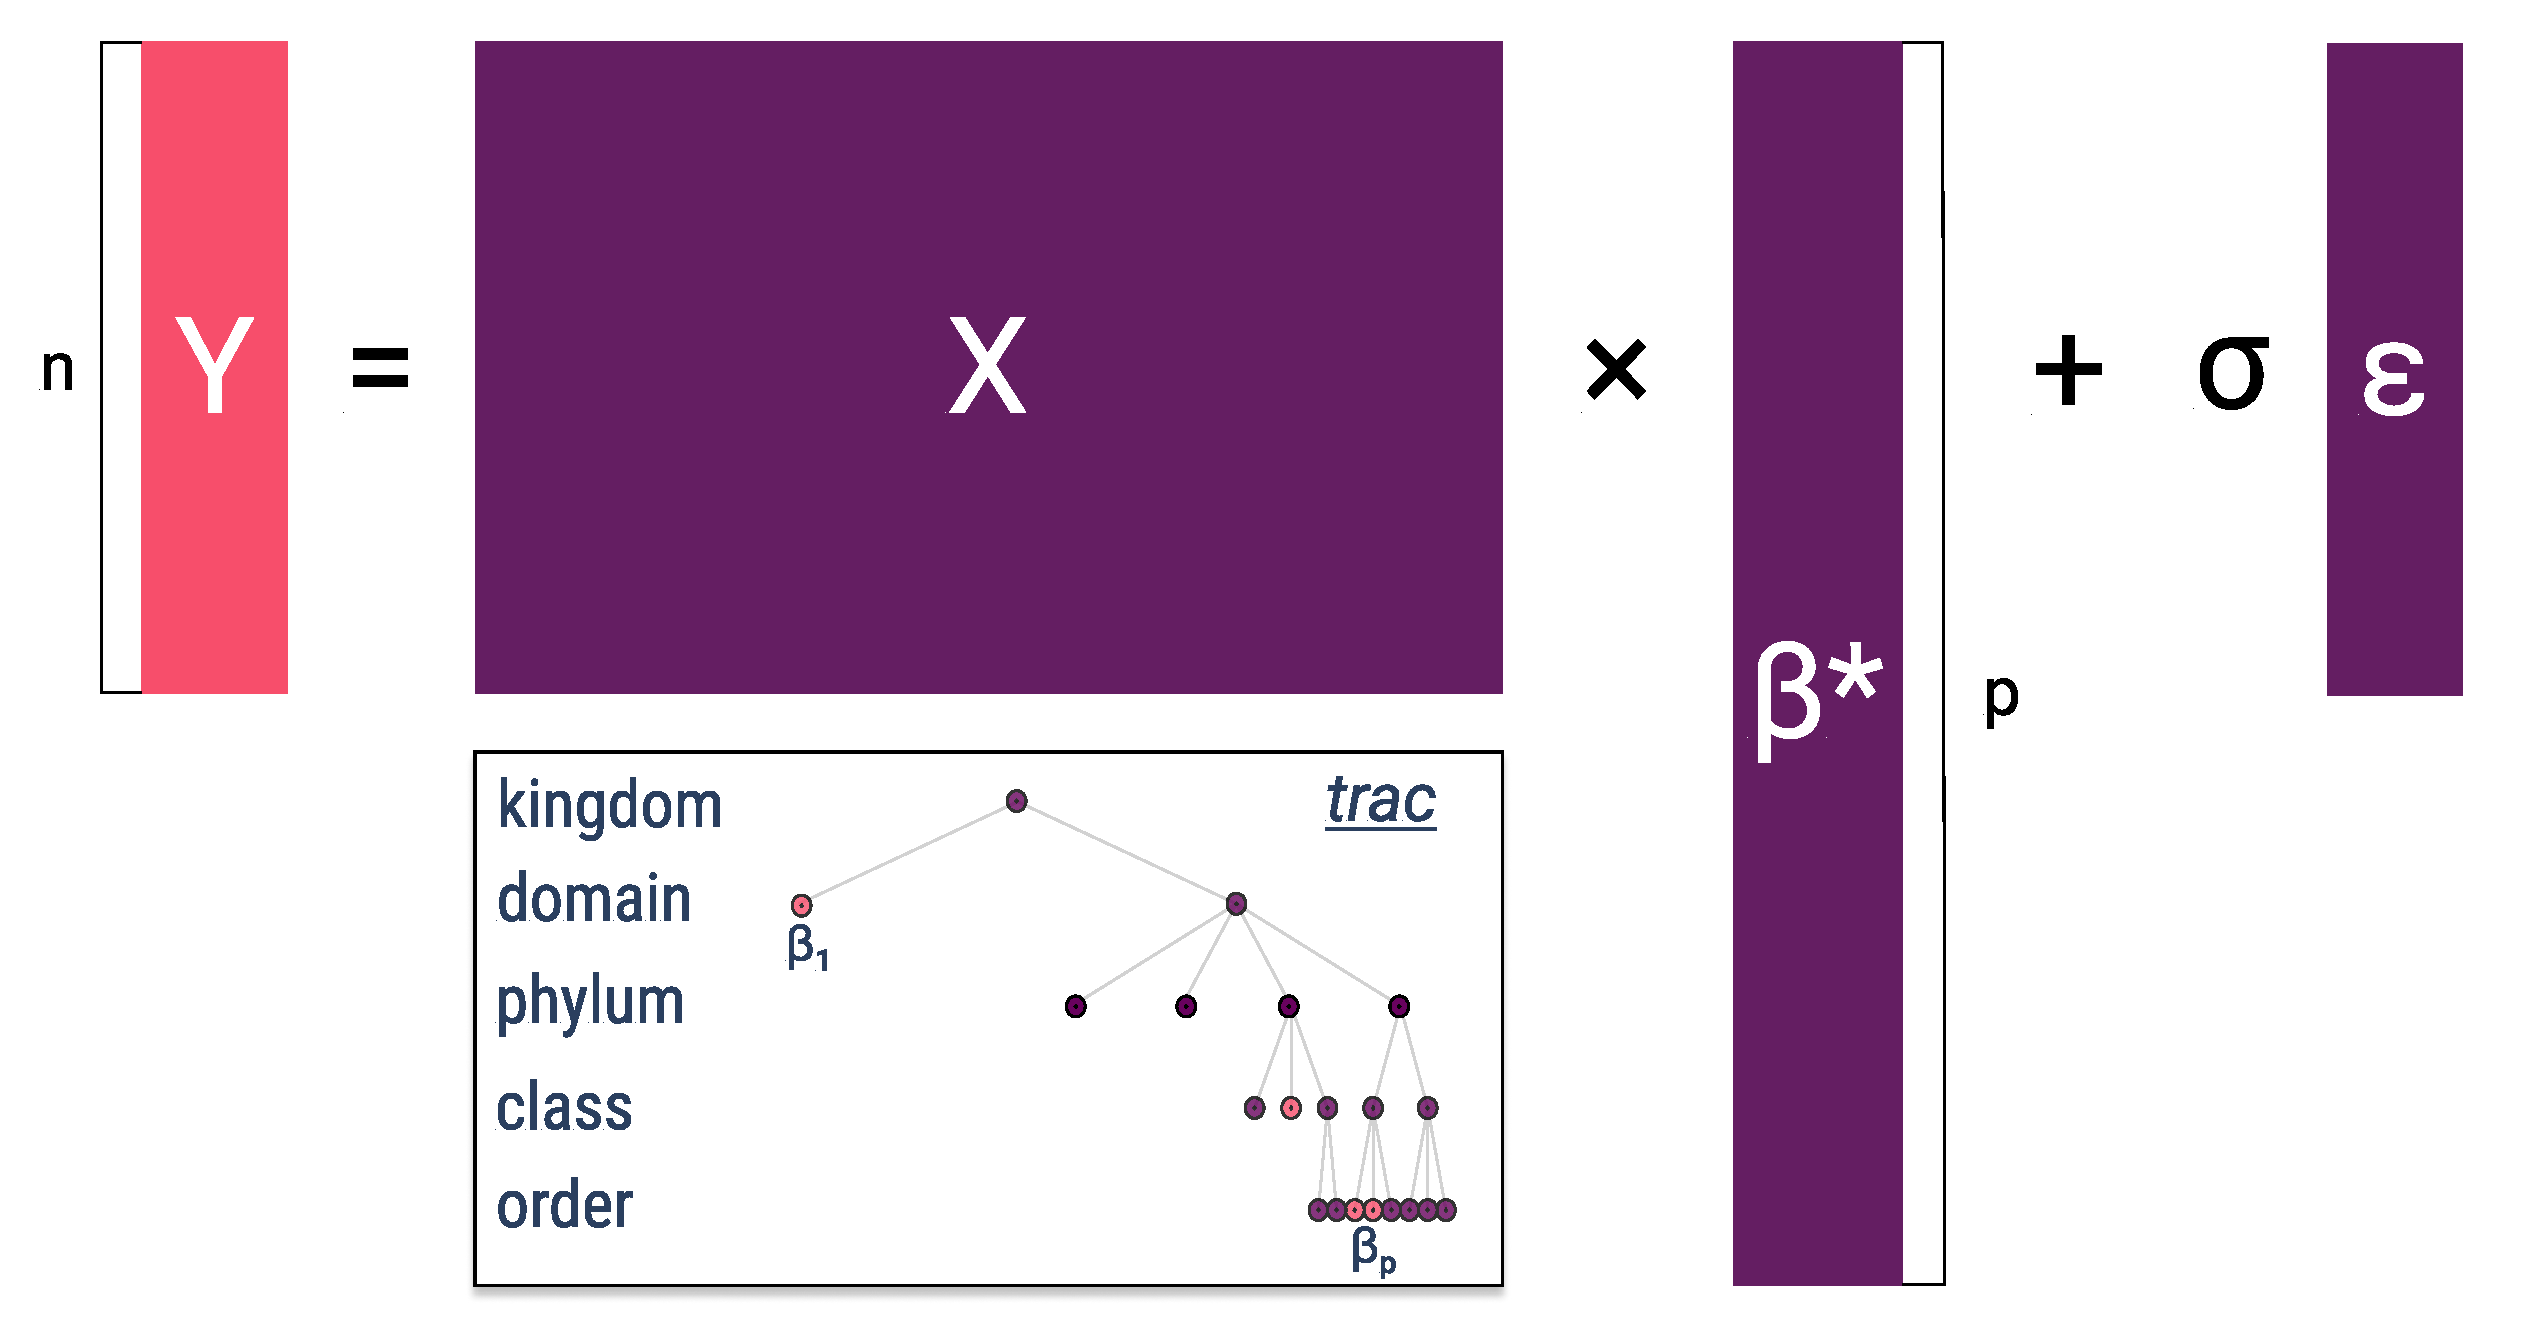
\includegraphics[width=0.65\linewidth]{figures/q2/slc_fig.pdf}
    \caption{High-demensional linear regression.}
    \label{fig:slc}
\end{figure}

\begin{figure}[h]
    \centering
    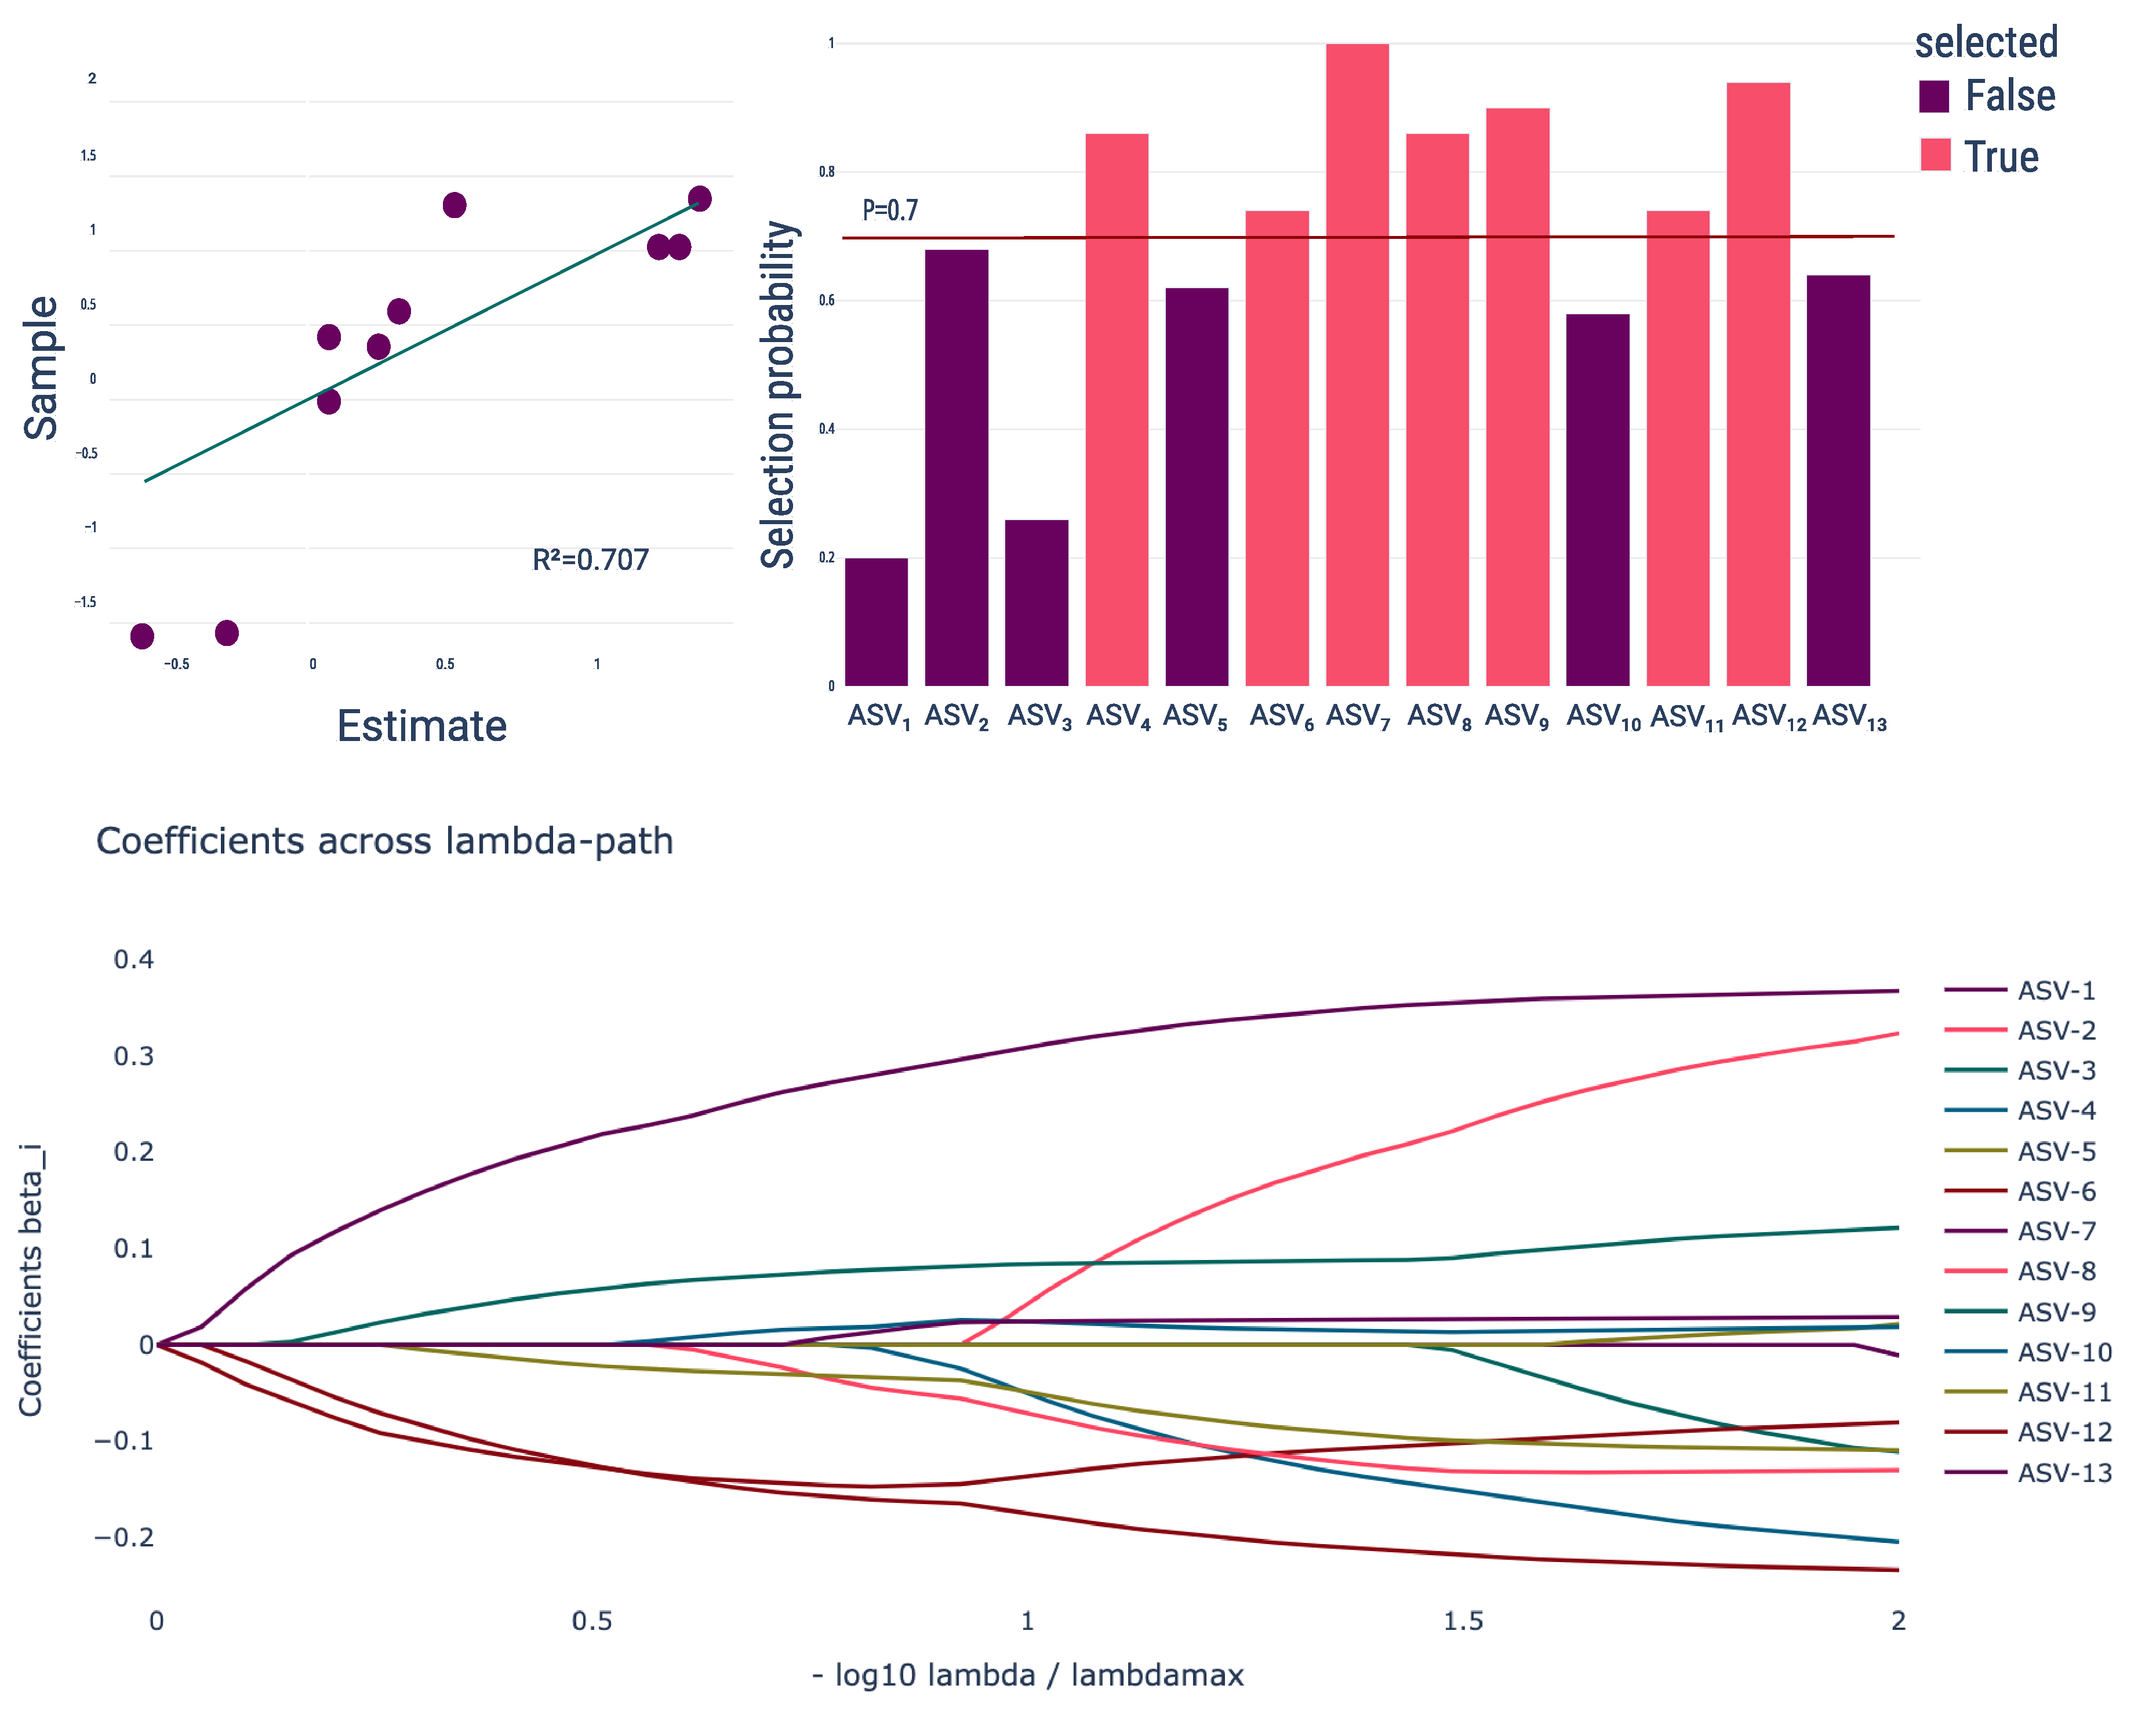
\includegraphics[width=0.85\linewidth]{figures/q2/reg.pdf}
    \caption{Standard constrained Lasso regression with stability selection.}
    \label{fig:acm_reg}
\end{figure}

Similarly, we can solve a classification task to predict a binary vegetation variable. We use the same set of covariates and microbial compositions, but the problem is now defined by \autoref{eq:slc}. In this example, we would like to use cross-validation as the model selection procedure, an option provided by q2-classo which complements the previously described stability selection approach. \autoref{fig:acm_class} shows the misclassification rate of the model as well as the refitted coefficients of $\beta$ after cross-validation with $\lambda=0.376$. From the summary statistics of the solution, we can compute standard metrics to assess and evaluate the performance of the model. The observed accuracy ($0.9$) signifies that 90\% of the model's predictions are accurate. Precision ($1$) implies an absence of false positives and recall ($0.8$) suggests a comparatively low incidence of false negatives. F1-score ($0.889$) is the harmonic mean of precision and is particularly useful in our case with uneven class distribution. Overall, these metrics suggest a reasonably good model where the most substantial contributions to vegetation prediction come from $ASV_{6}$ and $ASV_{9}$ which are also linked to the temperature. 

% \captionof{equation}{Sparse log-contrast regression:

% where Y is the average soil temperature.}
% \label{eq:sparse_log_contrast}

\begin{figure}[h]
    \centering
    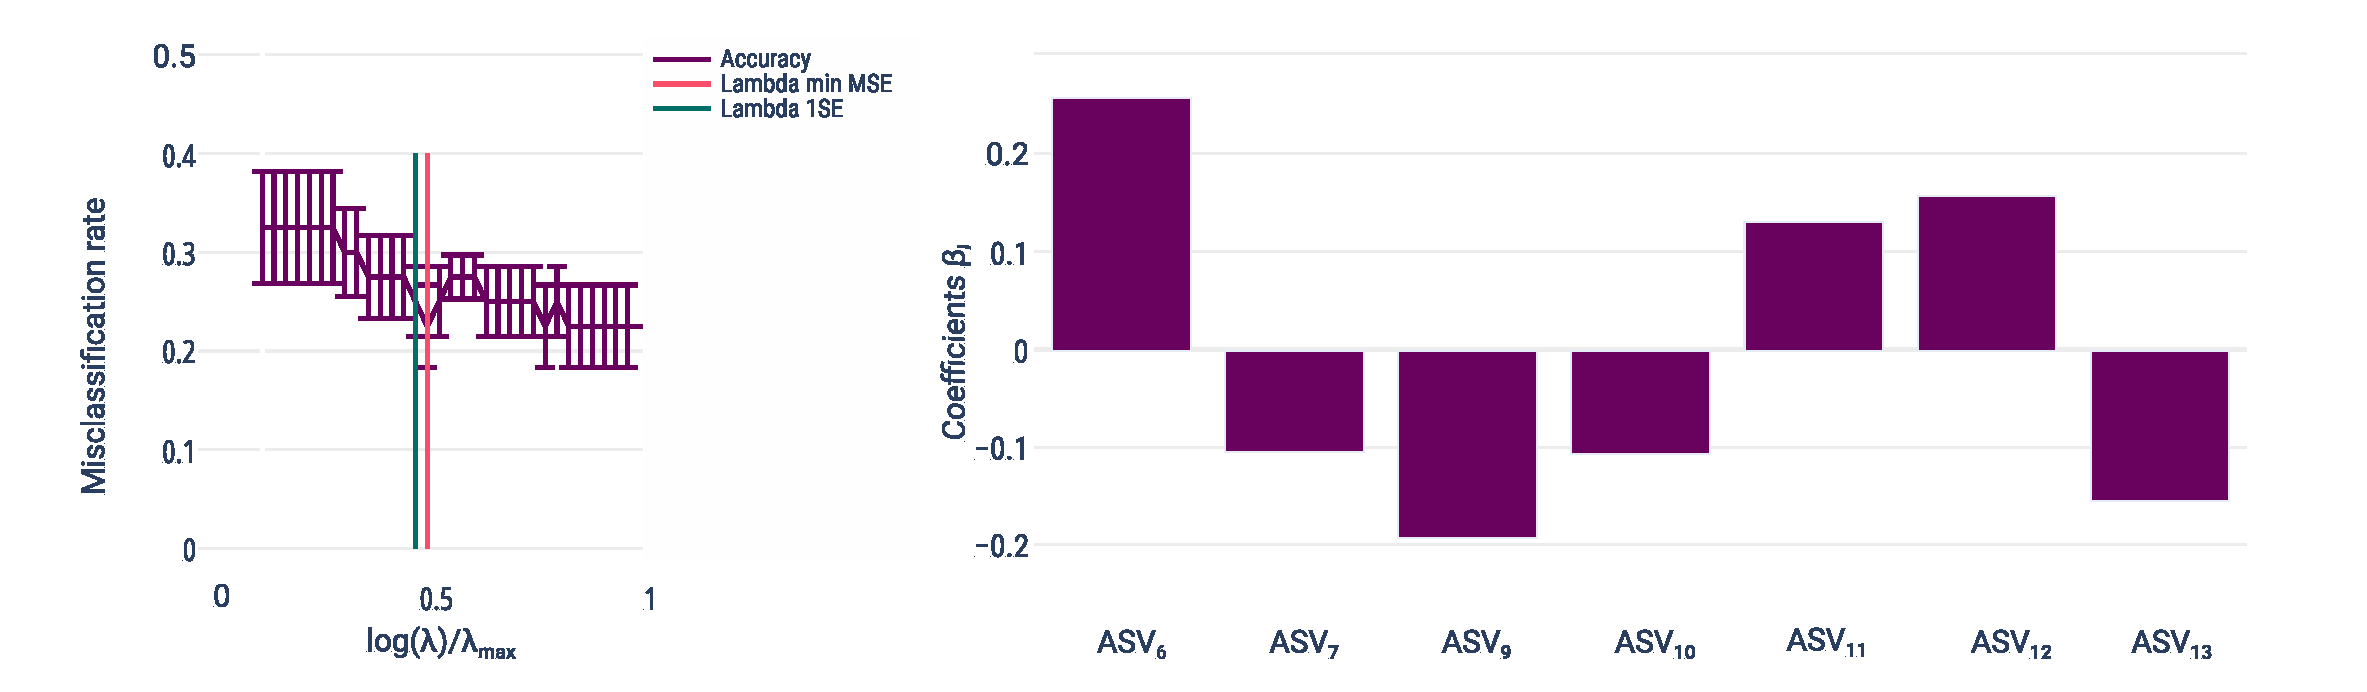
\includegraphics[width=\linewidth]{figures/q2/classo_class.pdf}
    \caption{Standard constrained Lasso classification with cross-validation.}
    \label{fig:acm_class}
\end{figure}




q2-classo also supports a combination of log-contrast regression and tree-aggregated regularization models \cite{bien2021tree}. The goal of these models is to utilize the taxonomic information from microbiome data (  \autoref{fig:slc}). Employing trac-models revealed marginally superior results in a regression context ($R^2=0.8$) but did not demonstrate any enhancement in the classification setting. Nevertheless, we recommend exploring trac-models, as it is common for the inclusion of taxonomic information to enhance model performance and interoperability.




% \begin{figure}[htbp]
%     \begin{minipage}{0.53\textwidth}
%         q2-classo also supports a combination of log-contrast regression and tree-aggregated regularization models \cite{bien2021tree}. The goal of these models is to utilize the taxonomic information from microbiome data (  \autoref{fig:acm_tree}). Employing trac-models revealed marginally superior results in a regression context ($R^2=0.8$) but did not demonstrate any enhancement in the classification setting. Nevertheless, we recommend exploring trac-models, as it is common for the inclusion of taxonomic information to enhance model performance and interpretability.
%      \end{minipage}%
%     \hfill 
%     \hspace{0.5cm}
%     \begin{minipage}{0.45\textwidth}
%         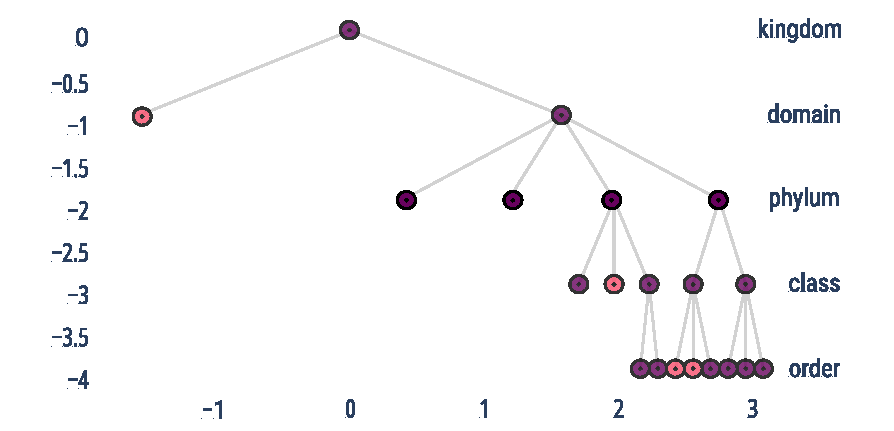
\includegraphics[width=\linewidth]{figures/q2/reg_tree.pdf}
%         \caption{Taxonomic tree.}
%         \label{fig:acm_tree}
%     \end{minipage}
% \end{figure}

\section*{Discussion} % Optional - only if novel data or analyses are included
% This section is only required if the paper includes novel data or analyses, and should be written in the same style as a traditional discussion section.
% Please include a brief discussion of allowances made (if any) for controlling bias or unwanted sources of variability, and the limitations of any novel datasets.


Microbiome data analysis presents a unique set of challenges due to its compositional, zero-inflated, overdispersed, and high-dimensional nature.
The compositional aspect arises from the fact that the abundance of individual taxa is expressed as proportions of the total microbial composition \cite{gloor2017microbiome}. The presence of zeros is a common phenomenon in microbiome data, where many taxa may be absent in certain samples. This zero-inflation introduces a hurdle in traditional statistical approaches, as methods assuming a continuous distribution may not be directly applicable. Furthermore, microbiome datasets often exhibit overdispersion, meaning that the variance of the counts is higher than expected under a Poisson or negative binomial distribution. The high-dimensional nature of microbiome data, characterized by a vast number of taxa or features, exacerbates the challenges. This abundance of variables can lead to increased computational demands and issues related to multiple testing, making it crucial to implement robust feature selection and dimensionality reduction techniques. While classification, regression, and network learning are classical machine learning tasks with various frameworks designed for their resolution, employing standard models may yield inaccurate outcomes due to the unique statistical challenges inherent in microbiome data. Therefore, we advocate for the adoption of our framework tailored to address these specific challenges in microbiome data analysis.


% Same as intro, but with the emphasis of what new have been done and why it is better to use this workdflow

% \section*{Conclusions} % Optional - only if novel data or analyses are included
% This section is only required if the paper includes novel data or analyses, and should be written as a traditional conclusion.




\section*{Data availability} % Required
% Use this section to provide the raw data that support their findings. Readers should be able to view the raw data, replicate the study, and re-analyse and/or reuse the data (with appropriate attribution). Please take a look at the F1000Research guidelines on \href{https://www.f1000research.com/for-authors/data-guidelines}{data preparation}.
% Raw data should be uploaded to an approved repository before submission, a list of which can be found on the \href{https://f1000research.com/for-authors/data-guidelines#hosting}{data guidelines page}.

% This section should be completed in the following format:

\subsection*{Source data}
The original Atacama soil microbiome data \cite{neilson2017significant} is available through the European Nucleotide Archive at the European Bioinformatics Institute (EMBL-EBI) under the accession number \href{https://www.ebi.ac.uk/ena/browser/view/PRJEB17617}{ERP019482}.

% If the data has been published previously, details of the dataset and where it can be accessed should be provided here.

\subsection*{Underlying data}

This project contains the following underlying data:
\begin{itemize}
	\item Count table of Atacama soil microbiome. (\autoref{tab:org_acm}.)
	\item Associated covariates of Atacama soil microbiome.
    \item Bacterial taxonomic annotations based on SILVA.
\end{itemize}

\begin{table}[h]
    \centering
    \caption{\label{tab:org_acm}Atacama soil microbiome data}
    \resizebox{\textwidth}{!}{
    \begin{tabular}{|l|*{13}{c|}}
        \hline
        & ASV-1 & ASV-2 & ASV-3 & ASV-4 & ASV-5 & ASV-6 & ASV-7 & ASV-8 & ASV-9 & ASV-10 & ASV-11 & ASV-12 & ASV-13 \\
        \hline
        BAQ2420.1.1 & 0.0 & 11.0 & 0.0 & 41.0 & 0.0 & 35.0 & 0.0 & 0.0 & 0.0 & 67.0 & 115.0 & 0.0 & 0.0 \\
        BAQ2420.1.2 & 0.0 & 0.0 & 0.0 & 26.0 & 17.0 & 45.0 & 0.0 & 59.0 & 0.0 & 20.0 & 0.0 & 0.0 & 0.0 \\
        BAQ2420.1.3 & 0.0 & 0.0 & 0.0 & 0.0 & 0.0 & 0.0 & 0.0 & 46.0 & 0.0 & 0.0 & 0.0 & 0.0 & 0.0 \\
        BAQ2420.2 & 0.0 & 7.0 & 0.0 & 0.0 & 0.0 & 0.0 & 0.0 & 37.0 & 0.0 & 0.0 & 0.0 & 30.0 & 0.0 \\
        BAQ2420.3 & 0.0 & 0.0 & 0.0 & 0.0 & 0.0 & 39.0 & 0.0 & 13.0 & 0.0 & 0.0 & 34.0 & 43.0 & 0.0 \\
        BAQ2462.1 & 0.0 & 11.0 & 0.0 & 9.0 & 0.0 & 65.0 & 0.0 & 0.0 & 0.0 & 0.0 & 0.0 & 47.0 & 0.0 \\
        BAQ2462.2 & 0.0 & 0.0 & 0.0 & 0.0 & 0.0 & 103.0 & 0.0 & 0.0 & 0.0 & 0.0 & 89.0 & 21.0 & 0.0 \\
        BAQ2462.3 & 0.0 & 9.0 & 0.0 & 0.0 & 0.0 & 24.0 & 0.0 & 0.0 & 0.0 & 0.0 & 44.0 & 71.0 & 0.0 \\
        BAQ2687.1 & 10.0 & 0.0 & 16.0 & 0.0 & 65.0 & 0.0 & 0.0 & 0.0 & 73.0 & 0.0 & 0.0 & 0.0 & 0.0 \\
        BAQ2687.2 & 0.0 & 0.0 & 0.0 & 0.0 & 0.0 & 34.0 & 0.0 & 0.0 & 0.0 & 0.0 & 91.0 & 0.0 & 0.0 \\
        BAQ2687.3 & 0.0 & 0.0 & 0.0 & 16.0 & 0.0 & 20.0 & 0.0 & 0.0 & 0.0 & 15.0 & 0.0 & 0.0 & 0.0 \\
        BAQ2838.1 & 0.0 & 0.0 & 0.0 & 9.0 & 0.0 & 16.0 & 21.0 & 0.0 & 0.0 & 42.0 & 0.0 & 49.0 & 0.0 \\
        BAQ2838.2 & 0.0 & 0.0 & 0.0 & 0.0 & 0.0 & 11.0 & 0.0 & 0.0 & 0.0 & 0.0 & 49.0 & 0.0 & 0.0 \\
        BAQ2838.3 & 0.0 & 0.0 & 0.0 & 0.0 & 0.0 & 0.0 & 0.0 & 0.0 & 0.0 & 23.0 & 0.0 & 14.0 & 0.0 \\
        BAQ3473.1 & 0.0 & 0.0 & 25.0 & 0.0 & 0.0 & 0.0 & 0.0 & 0.0 & 230.0 & 42.0 & 0.0 & 0.0 & 0.0 \\
        BAQ3473.2 & 0.0 & 0.0 & 0.0 & 17.0 & 39.0 & 0.0 & 12.0 & 0.0 & 65.0 & 62.0 & 0.0 & 0.0 & 65.0 \\
        BAQ3473.3 & 0.0 & 0.0 & 48.0 & 0.0 & 0.0 & 0.0 & 0.0 & 0.0 & 209.0 & 0.0 & 0.0 & 0.0 & 0.0 \\
        BAQ4166.1.1 & 0.0 & 0.0 & 10.0 & 0.0 & 0.0 & 0.0 & 16.0 & 0.0 & 0.0 & 0.0 & 0.0 & 0.0 & 0.0 \\
        BAQ4166.1.2 & 21.0 & 10.0 & 13.0 & 0.0 & 108.0 & 0.0 & 0.0 & 0.0 & 53.0 & 62.0 & 0.0 & 0.0 & 0.0 \\
        BAQ4166.1.3 & 7.0 & 0.0 & 0.0 & 0.0 & 65.0 & 0.0 & 0.0 & 0.0 & 0.0 & 118.0 & 0.0 & 0.0 & 0.0 \\
        BAQ4166.2 & 18.0 & 0.0 & 0.0 & 0.0 & 84.0 & 0.0 & 37.0 & 0.0 & 0.0 & 0.0 & 0.0 & 0.0 & 11.0 \\
        BAQ4166.3 & 0.0 & 0.0 & 13.0 & 0.0 & 76.0 & 0.0 & 22.0 & 0.0 & 0.0 & 111.0 & 0.0 & 0.0 & 24.0 \\
        BAQ4697.1 & 4.0 & 0.0 & 0.0 & 0.0 & 0.0 & 0.0 & 66.0 & 0.0 & 122.0 & 17.0 & 0.0 & 0.0 & 0.0 \\
        BAQ4697.2 & 0.0 & 0.0 & 0.0 & 0.0 & 0.0 & 0.0 & 74.0 & 0.0 & 31.0 & 38.0 & 0.0 & 0.0 & 0.0 \\
        BAQ4697.3 & 0.0 & 0.0 & 0.0 & 0.0 & 0.0 & 0.0 & 65.0 & 0.0 & 48.0 & 50.0 & 0.0 & 0.0 & 0.0 \\
        YUN1242.1 & 0.0 & 0.0 & 0.0 & 0.0 & 0.0 & 0.0 & 0.0 & 0.0 & 0.0 & 0.0 & 19.0 & 23.0 & 0.0 \\
        YUN1242.3 & 0.0 & 0.0 & 0.0 & 0.0 & 0.0 & 35.0 & 0.0 & 0.0 & 0.0 & 0.0 & 110.0 & 175.0 & 0.0 \\
        YUN1609.1 & 0.0 & 0.0 & 0.0 & 0.0 & 0.0 & 33.0 & 0.0 & 0.0 & 0.0 & 0.0 & 61.0 & 771.0 & 0.0 \\
        YUN2029.2 & 0.0 & 0.0 & 0.0 & 0.0 & 0.0 & 27.0 & 0.0 & 0.0 & 0.0 & 0.0 & 260.0 & 0.0 & 0.0 \\
        YUN3153.2 & 0.0 & 11.0 & 0.0 & 0.0 & 0.0 & 24.0 & 0.0 & 0.0 & 0.0 & 8.0 & 119.0 & 0.0 & 0.0 \\
        YUN3153.3 & 0.0 & 8.0 & 0.0 & 0.0 & 0.0 & 12.0 & 0.0 & 0.0 & 0.0 & 6.0 & 112.0 & 0.0 & 0.0 \\
        YUN3259.1.2 & 0.0 & 0.0 & 0.0 & 12.0 & 0.0 & 0.0 & 39.0 & 15.0 & 0.0 & 51.0 & 0.0 & 23.0 & 0.0 \\
        YUN3259.1.3 & 0.0 & 0.0 & 0.0 & 5.0 & 0.0 & 0.0 & 0.0 & 0.0 & 0.0 & 0.0 & 0.0 & 0.0 & 0.0 \\
        YUN3259.2 & 0.0 & 0.0 & 0.0 & 19.0 & 0.0 & 14.0 & 42.0 & 0.0 & 46.0 & 59.0 & 0.0 & 22.0 & 0.0 \\
        YUN3259.3 & 0.0 & 25.0 & 0.0 & 26.0 & 9.0 & 0.0 & 0.0 & 0.0 & 0.0 & 48.0 & 0.0 & 20.0 & 0.0 \\
        YUN3346.1 & 0.0 & 0.0 & 0.0 & 0.0 & 0.0 & 17.0 & 0.0 & 0.0 & 0.0 & 25.0 & 0.0 & 18.0 & 0.0 \\
        YUN3346.2 & 0.0 & 0.0 & 0.0 & 0.0 & 0.0 & 0.0 & 0.0 & 0.0 & 0.0 & 0.0 & 0.0 & 0.0 & 53.0 \\
        YUN3346.3 & 0.0 & 0.0 & 0.0 & 0.0 & 0.0 & 12.0 & 0.0 & 0.0 & 0.0 & 28.0 & 54.0 & 0.0 & 70.0 \\
        YUN3428.1 & 0.0 & 0.0 & 0.0 & 0.0 & 0.0 & 0.0 & 18.0 & 75.0 & 0.0 & 0.0 & 0.0 & 0.0 & 0.0 \\
        YUN3428.2 & 0.0 & 0.0 & 39.0 & 9.0 & 0.0 & 13.0 & 14.0 & 62.0 & 0.0 & 0.0 & 0.0 & 0.0 & 0.0 \\
        YUN3533.1.2 & 10.0 & 0.0 & 10.0 & 0.0 & 0.0 & 17.0 & 9.0 & 70.0 & 43.0 & 0.0 & 0.0 & 0.0 & 91.0 \\
        YUN3533.1.3 & 0.0 & 0.0 & 0.0 & 0.0 & 0.0 & 0.0 & 0.0 & 35.0 & 0.0 & 0.0 & 0.0 & 0.0 & 174.0 \\
        YUN3533.2 & 9.0 & 14.0 & 15.0 & 0.0 & 0.0 & 0.0 & 11.0 & 38.0 & 0.0 & 76.0 & 0.0 & 0.0 & 58.0 \\
        YUN3533.3 & 17.0 & 17.0 & 0.0 & 0.0 & 0.0 & 0.0 & 30.0 & 65.0 & 0.0 & 74.0 & 0.0 & 0.0 & 134.0 \\
        YUN3856.1.1 & 0.0 & 0.0 & 0.0 & 0.0 & 0.0 & 0.0 & 54.0 & 0.0 & 0.0 & 0.0 & 0.0 & 0.0 & 0.0 \\
        YUN3856.1.2 & 18.0 & 16.0 & 0.0 & 24.0 & 19.0 & 0.0 & 26.0 & 64.0 & 0.0 & 0.0 & 0.0 & 0.0 & 598.0 \\
        YUN3856.1.3 & 0.0 & 0.0 & 0.0 & 0.0 & 0.0 & 0.0 & 0.0 & 0.0 & 66.0 & 0.0 & 28.0 & 27.0 & 0.0 \\
        YUN3856.2 & 6.0 & 13.0 & 26.0 & 45.0 & 16.0 & 0.0 & 25.0 & 0.0 & 0.0 & 70.0 & 0.0 & 0.0 & 104.0 \\
        YUN3856.3 & 21.0 & 36.0 & 23.0 & 31.0 & 34.0 & 0.0 & 22.0 & 77.0 & 0.0 & 0.0 & 33.0 & 0.0 & 0.0 \\
        \hline
    \end{tabular}
    }
\end{table}

% \begin{figure}[!h]
%     \centering
%     \begin{subfigure}[b]{0.4\linewidth}
%         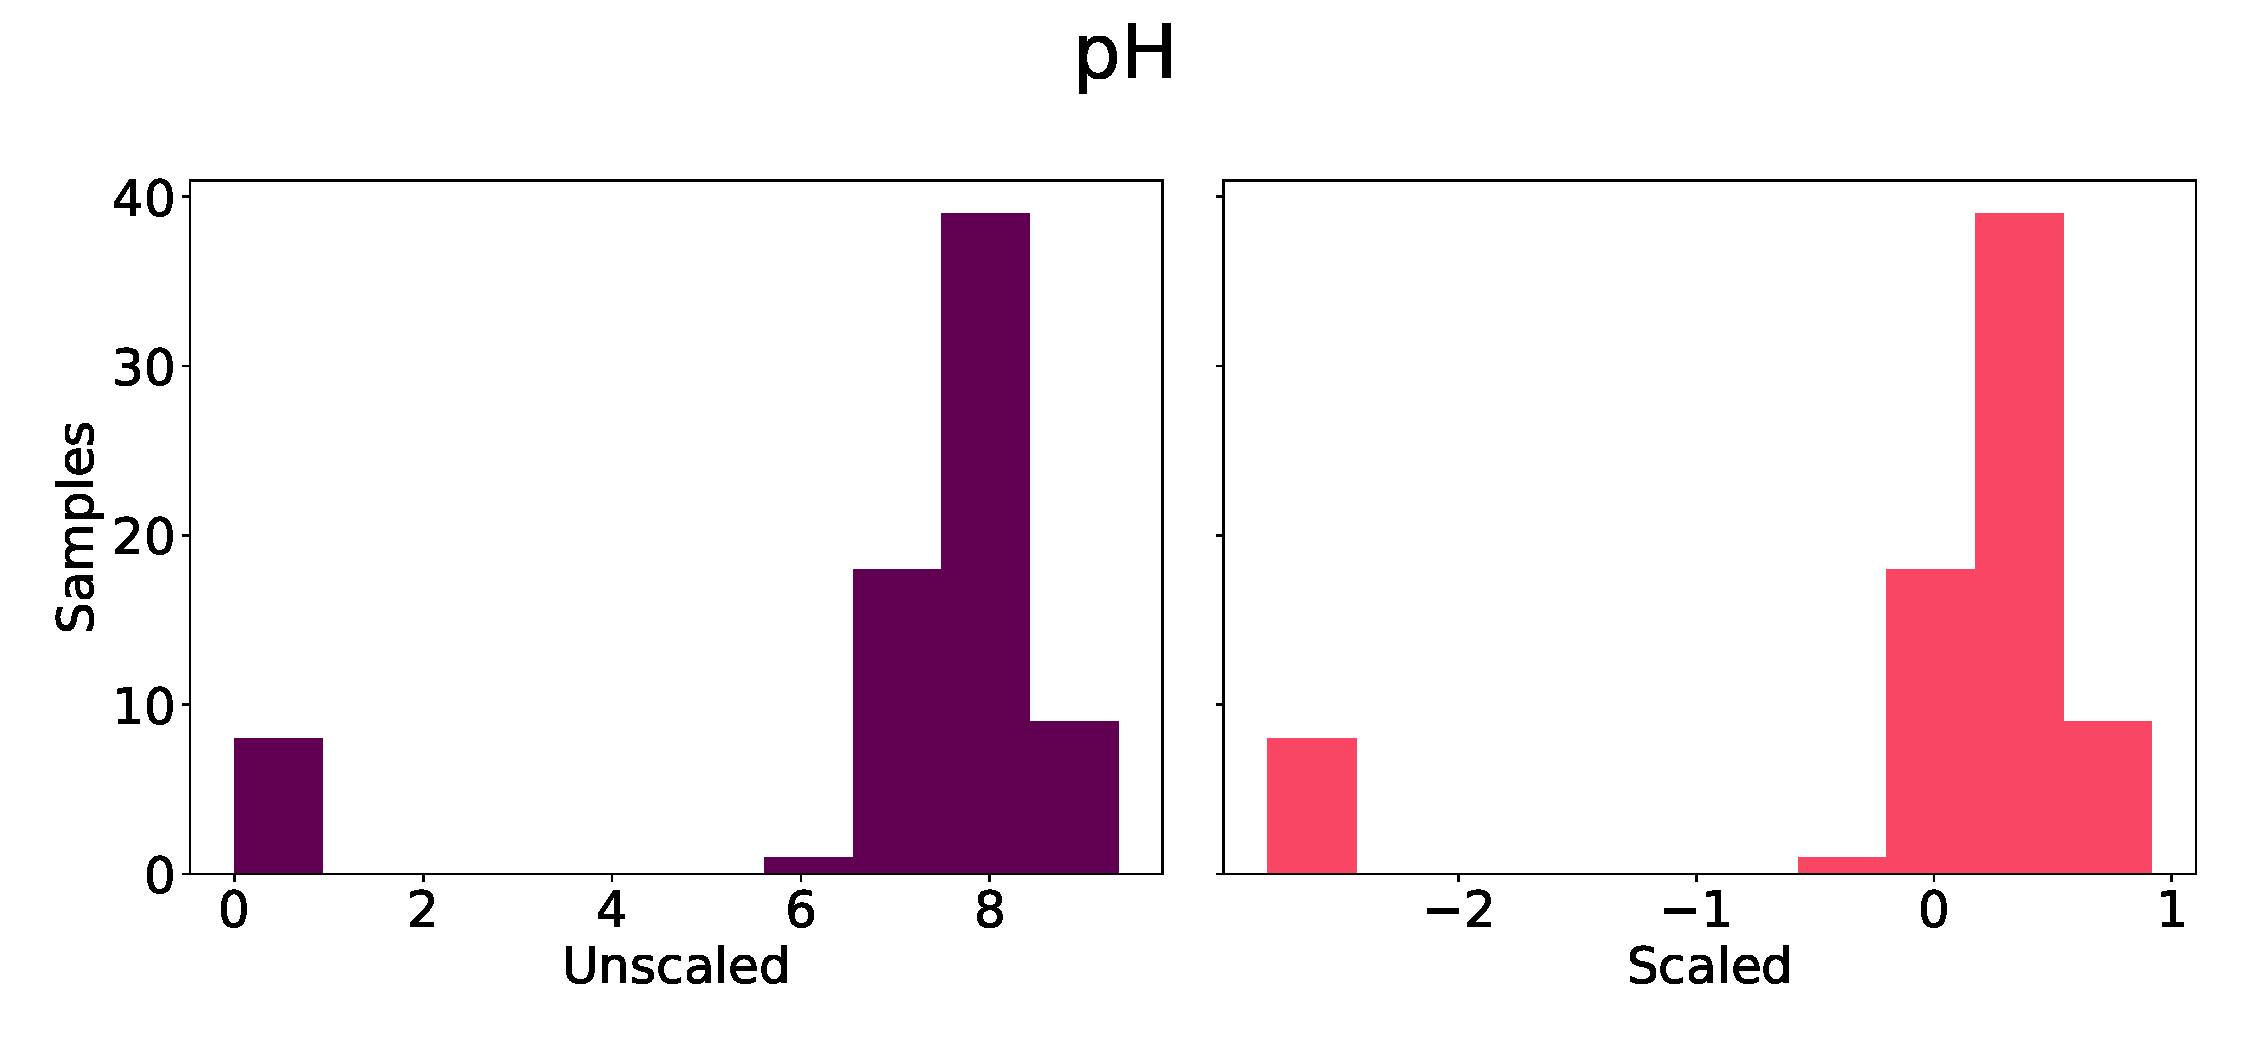
\includegraphics[width=\linewidth]{figures/q2/ph.pdf}
%         \label{fig:ph}
%     \end{subfigure}
%     \begin{subfigure}[b]{0.4\linewidth}
%         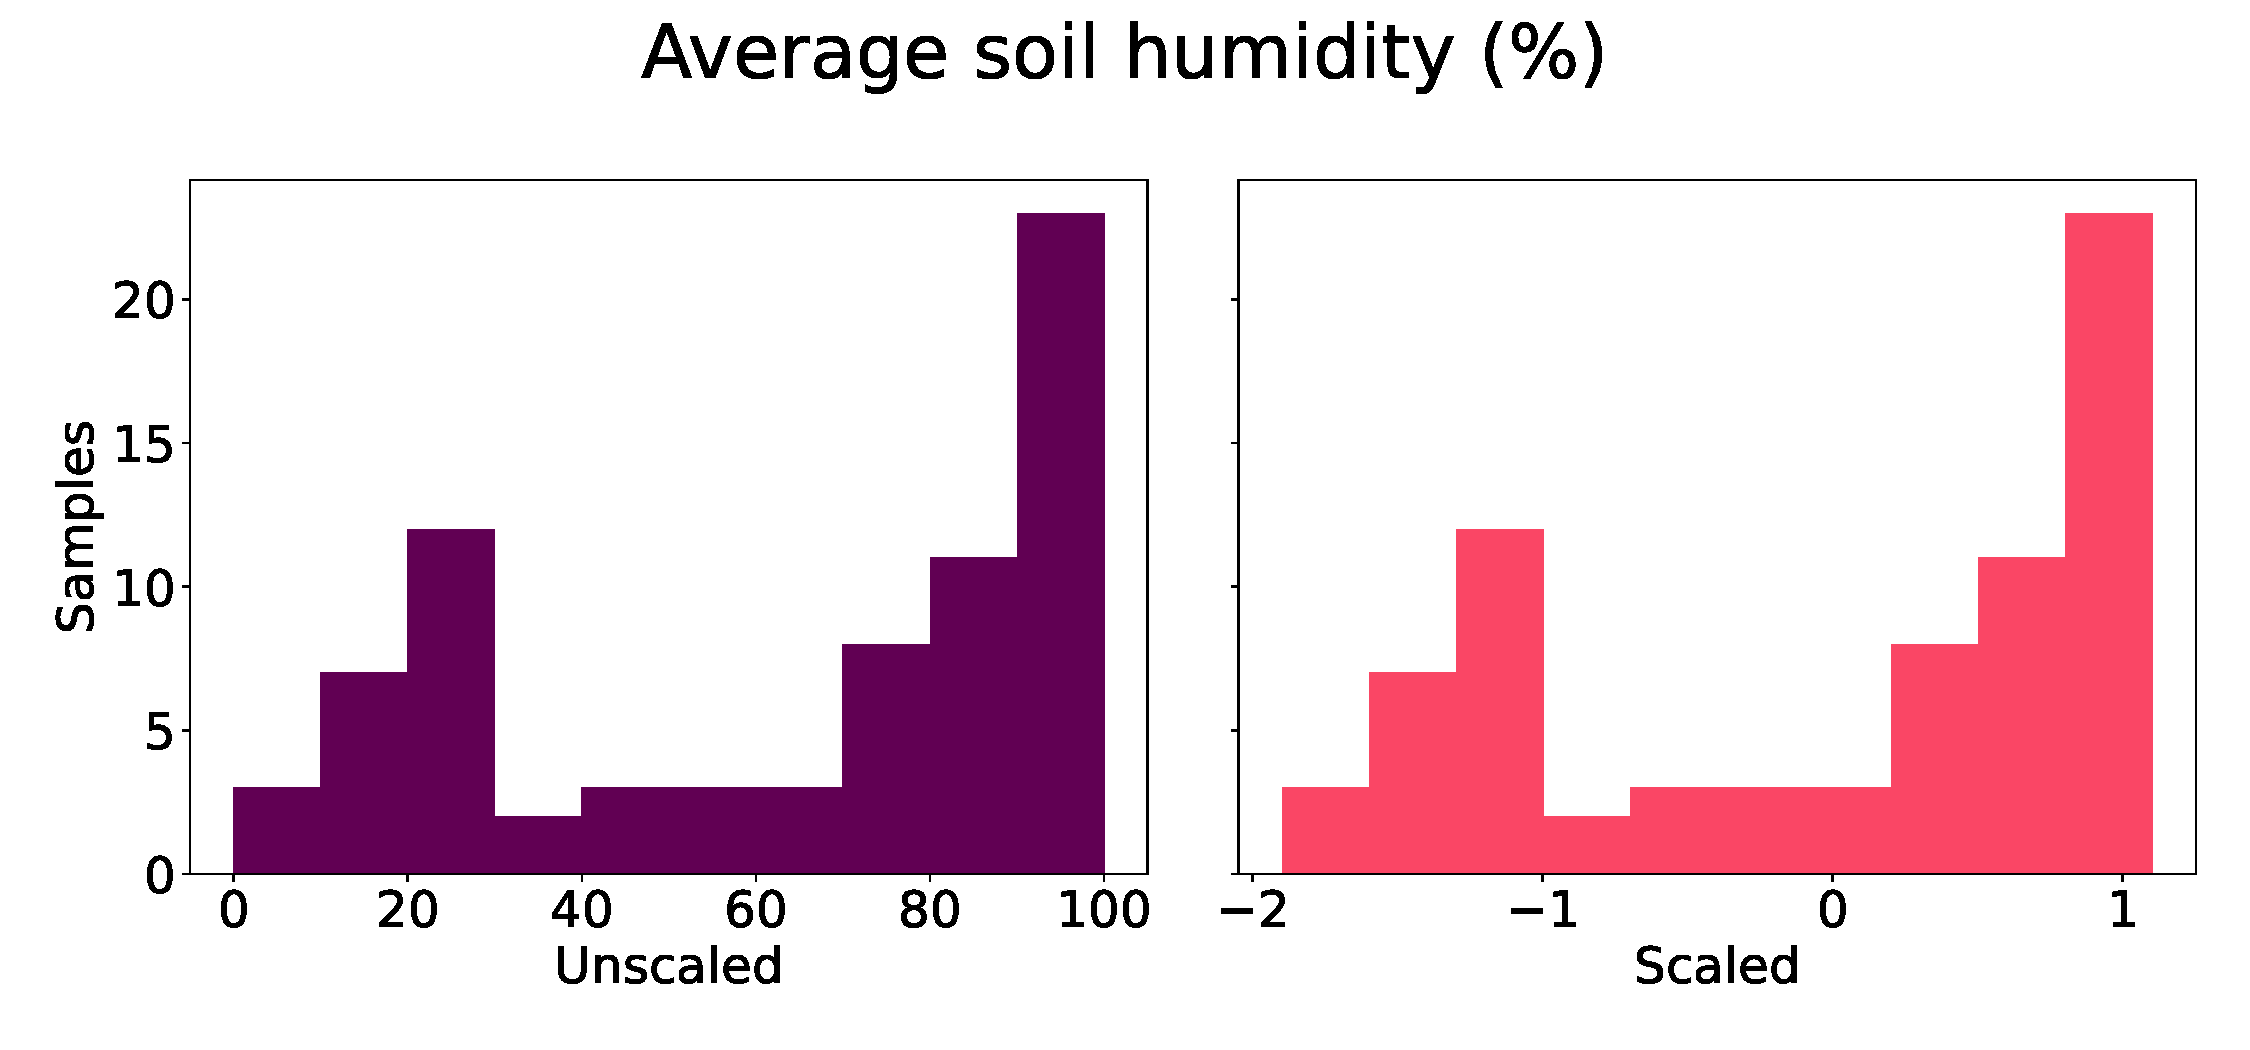
\includegraphics[width=\linewidth]{figures/q2/average-soil-relative-humidity.pdf}
%         \label{fig:humidity}
%     \end{subfigure}
%     \begin{subfigure}[b]{0.4\linewidth}
%         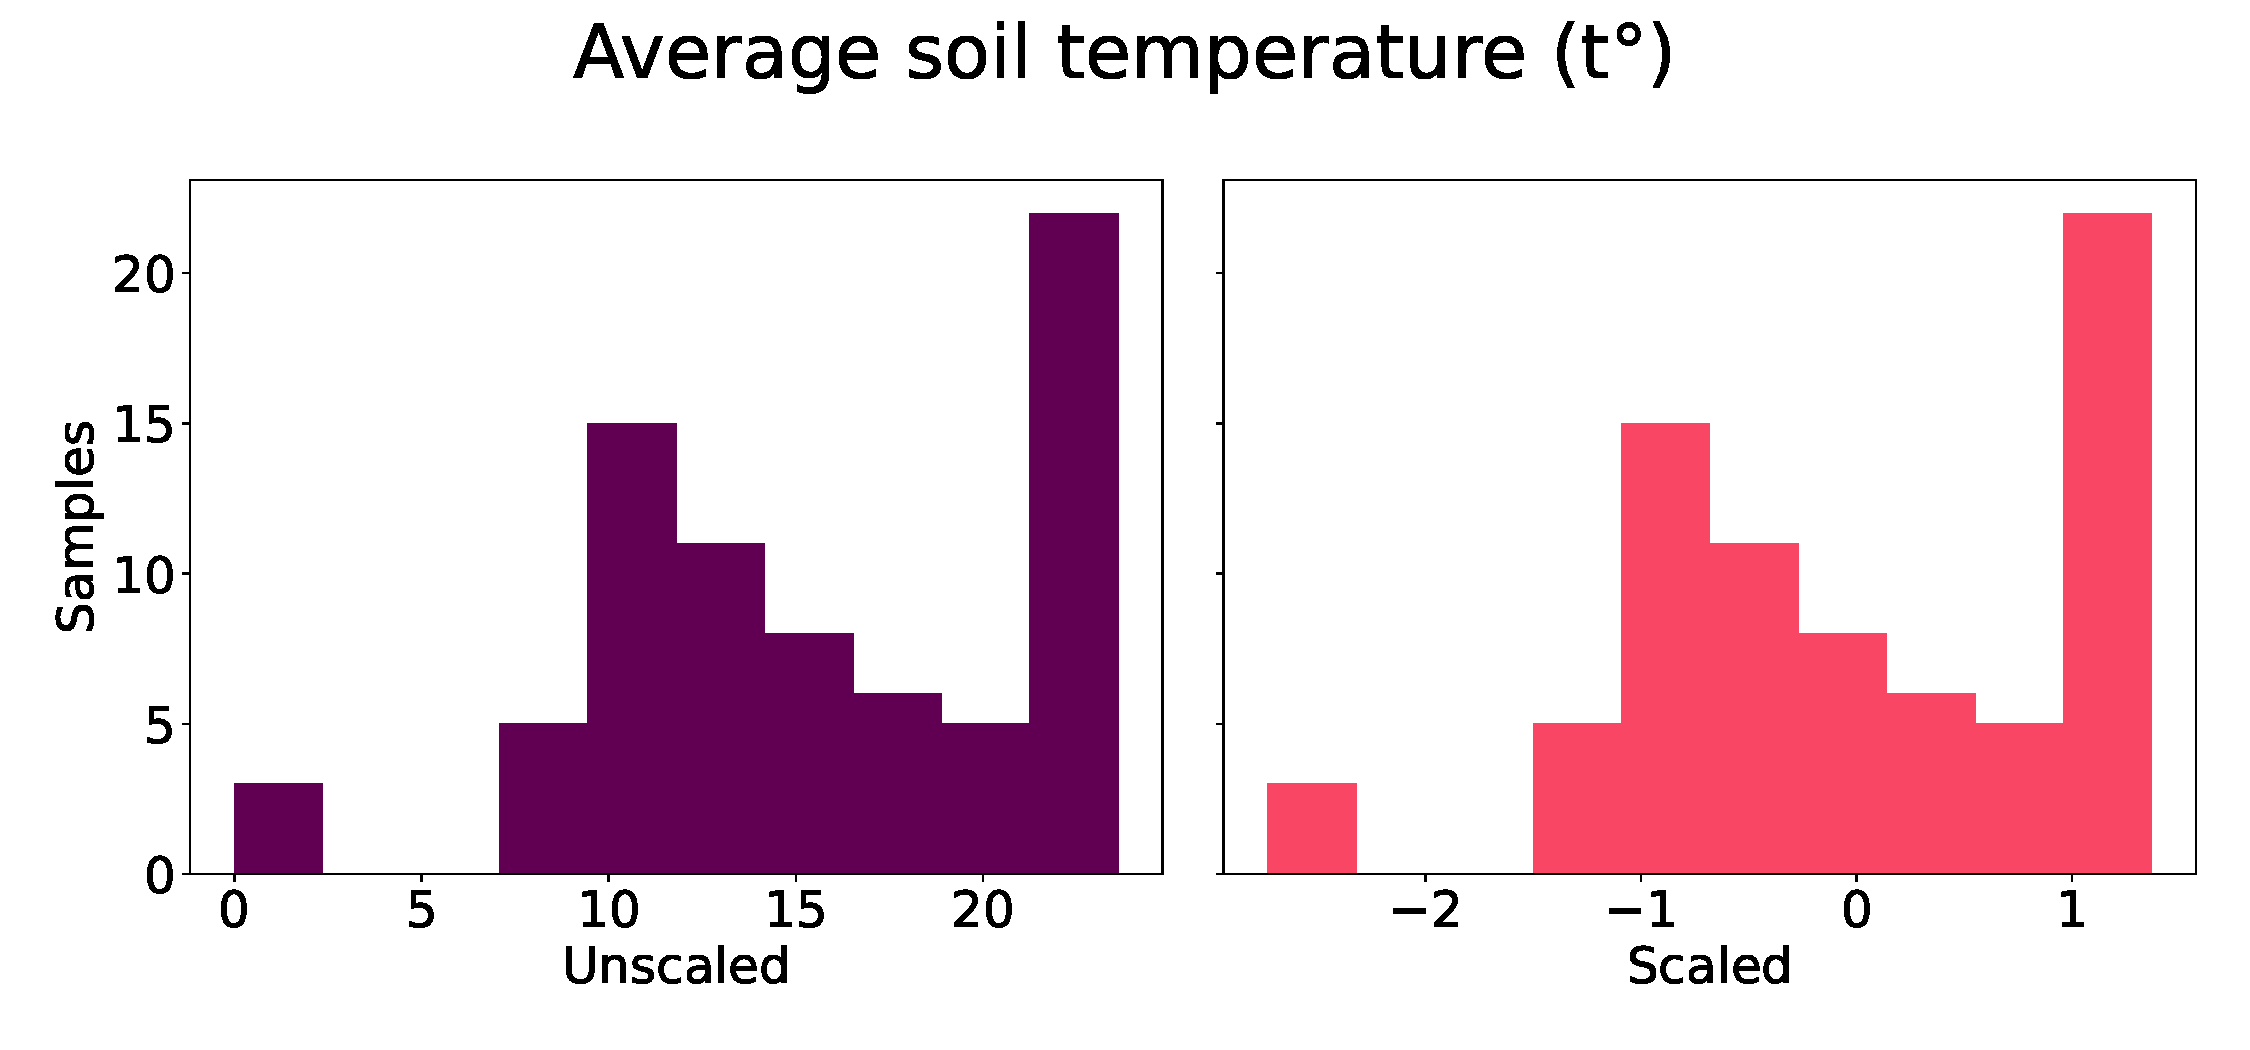
\includegraphics[width=\linewidth]{figures/q2/average-soil-temperature.pdf}
%         \label{fig:temp}
%     \end{subfigure}
%     \begin{subfigure}[b]{0.4\linewidth}
%         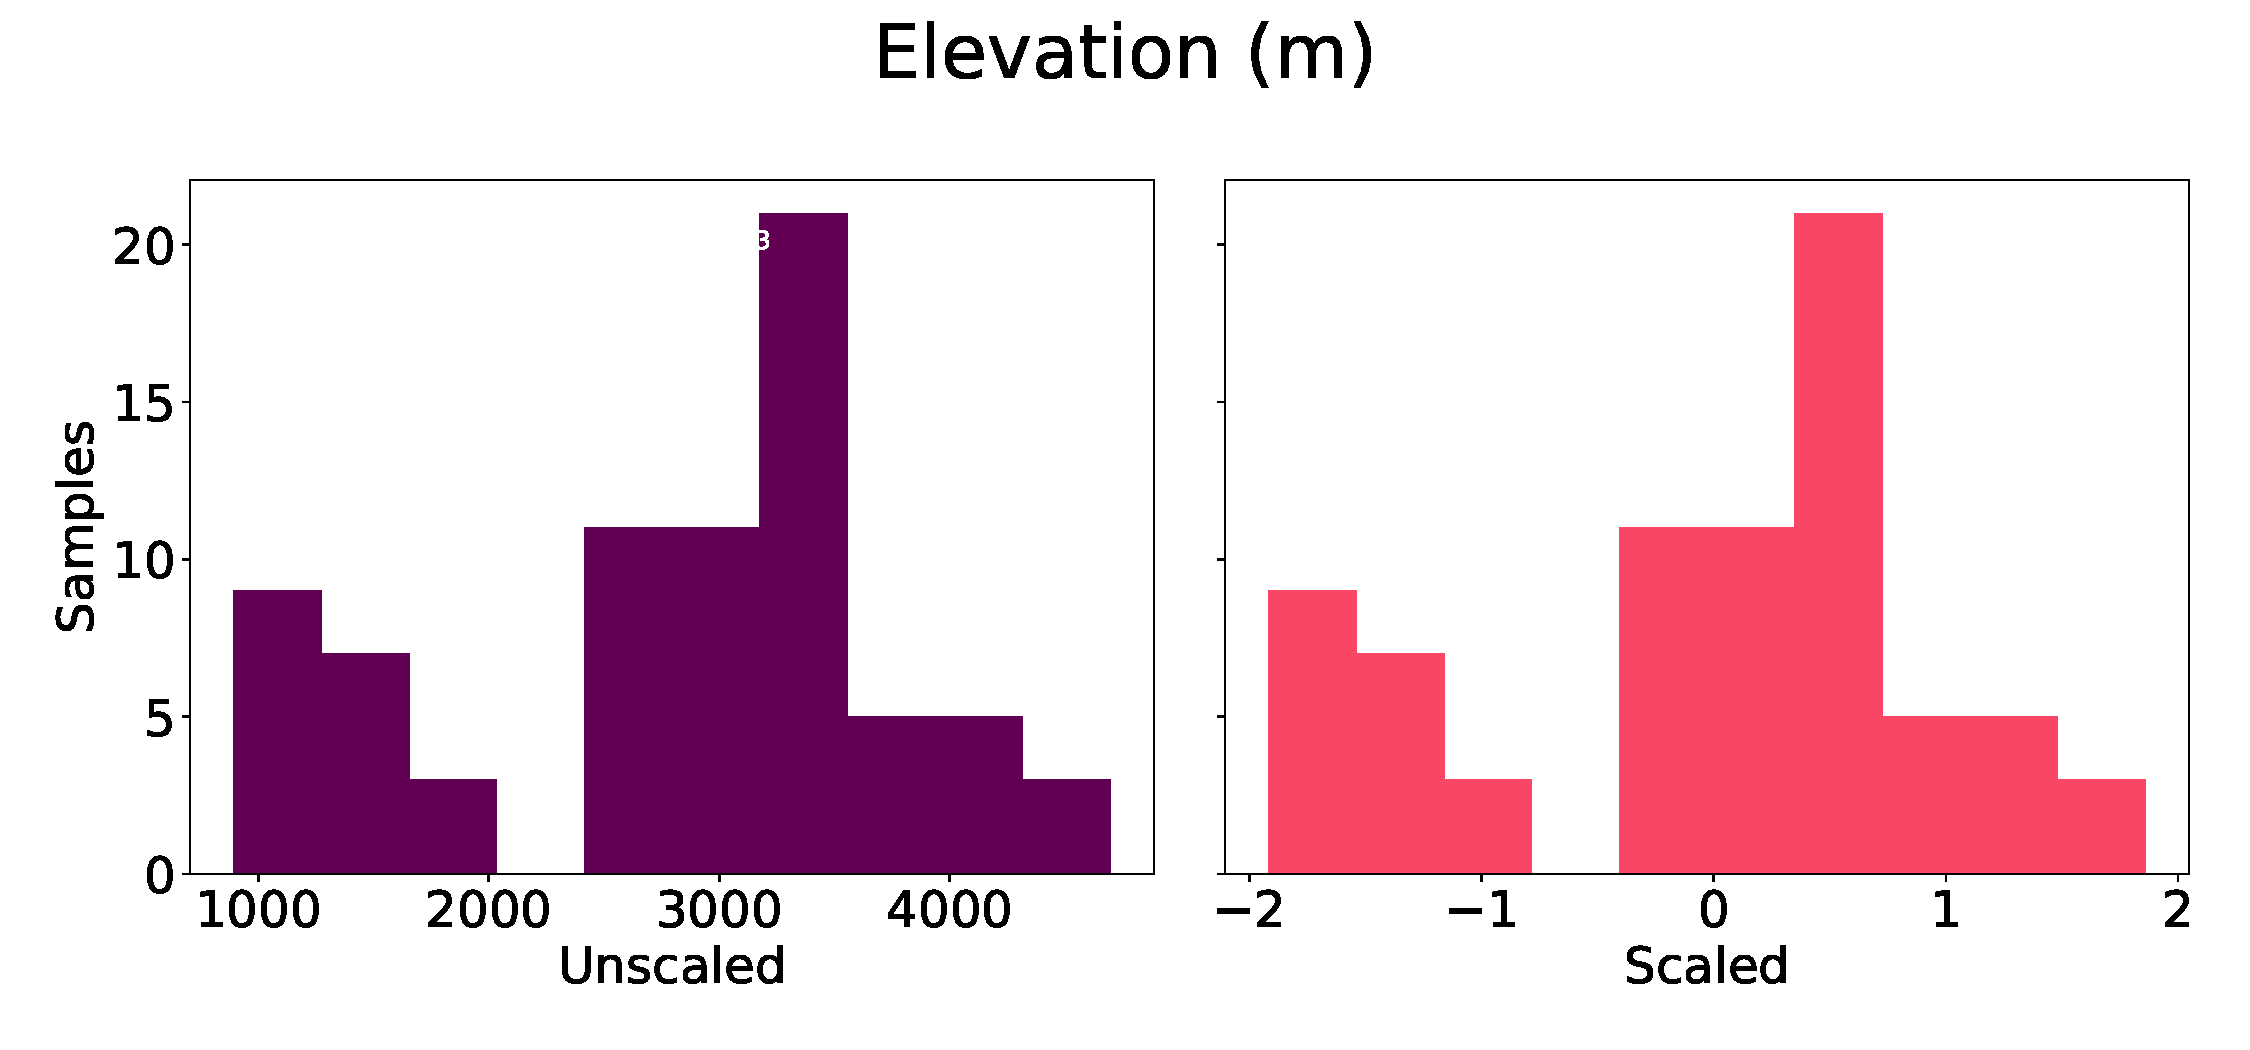
\includegraphics[width=\linewidth]{figures/q2/elevation.pdf}
%         \label{fig:elevation}
%     \end{subfigure}
%     \caption{Scaled covariates associated with Atacama soil microbiome.}
%     \label{fig:acm_covariates}
% \end{figure}

% This section should detail all novel data collected and used as part of your article. Details of the repository where your data are hosted, a description of the data files and the license under which they are held should be included. See the F1000Research Data Guidelines for more information. The following formatting should be used:
% \begin{quote}
% Repository: Manually annotated miRNA-disease and miRNA-gene interaction corpora.\\
% https://doi.org/10.5256/repository.4591.d34639.
% \\
% \\


% Data are available under the terms of the Creative Commons Zero "No rights reserved" data waiver (CC0 1.0 Public domain dedication).
% \end{quote}


% \subsection*{Extended data}

% Additional materials that support the key claims in the paper but are not absolutely required to follow the study design and analysis of the results (e.g. questionnaires, supporting images or tables) should be included as extended data. Details of the repository where these materials are hosted, a description of the extended data files and the license under which they are held should be included. See the F1000Research Data Guidelines for more information.






\section*{Software availability}
% Source code for new software must be made openly and permanently available in a structured repository such as Zenodo (see ‘Making Your Code Citable’ for more information), and assigned an open license; we strongly encourage the use of an OSS approved license, but will accept other open licenses including Creative Commons. The Software availability section must include the following information:

Both plugins have been previously implemented in Python and now can also be installed from QIIME2 or \href{https://hub.docker.com}{Docker Hub}. For a specific problem formulation and more examples, we encourage you to visit \href{https://gglasso--37.org.readthedocs.build/en/37/getting-started.html}{gglasso} and \href{https://c-lasso.readthedocs.io/en/latest/index.html}{classo} documentation.

\begin{itemize}
	\item Software available from QIIME2: https://qiime2.org/
	\item Source code available from GitHub: https://github.com/Vlasovets/q2-gglasso
    \item Source code available from GitHub: https://github.com/Leo-Simpson/q2-classo
	\item Archived source code at time of publication: DOI for archived source code
	\item License: MIT License
\end{itemize}

\section*{Competing interests}
No competing interests were disclosed
% All financial, personal, or professional competing interests for any of the authors that could be construed to unduly influence the content of the article must be disclosed and will be displayed alongside the article. If there are no relevant competing interests to declare, please add the following: 'No competing interests were disclosed'.

\section*{Grant information}
The author(s) declared that no grants were involved in supporting this work.
% Please state who funded the work discussed in this article, whether it is your employer, a grant funder etc. Please do not list funding that you have that is not relevant to this specific piece of research. For each funder, please state the funder’s name, the grant number where applicable, and the individual to whom the grant was assigned.
% If your work was not funded by any grants, please include the line: ‘The author(s) declared that no grants were involved in supporting this work.’

\section*{Acknowledgements}
This project is supported by the Munich School for Data Science (\href{https://www.mu-ds.de/}{MUDS}).


{\small\bibliographystyle{unsrtnat}
\bibliography{sample}}

% Include a reference list in your .tex file - if using a .bib file this can be generated with \textbackslash bibliography as demonstrated above. References can be listed in any standard referencing style and should be consistent between references within a given article. In-line references should be formatted using \textbackslash cite, for example \cite{Smith:2012qr} and \cite{Smith:2013jd} 


% \section*{Using LaTeX}
% In order to ensure smooth and successful processing of your LaTeX manuscript, please follow these guidelines. Before submitting ensure that your PDF appears correctly on Overleaf, to avoid delays in processing. You can view and outstanding errors on the Logs and Output Files tab, just to the right of the green Recompile button.

% As you prepare your LaTeX manuscript, please bear in mind the following general guidelines.  
% Keep it simple:

% \begin{enumerate}
%     \item[~]
% 	\begin{enumerate}
% 		\item Keep your LaTeX files as simple as possible; do not use elaborate local macros or highly customized style files. Preferably, use the template provided for formatting your paper.
% 		\item Preferably prepare only one .tex file. 
% 		\item Do not use external style files or packages, except for f1000styles.sty and those packages already referenced in the main.tex template. If you need additional macros, please keep them simple and include them in the .tex document preamble.
% 		\item Source code should be structured so that all .sty and .bst files called by the main .tex file are in the same directory as the main .tex file.
% 		\item AMS math commands are recommended when inserting math equations into your manuscript.
% 		\item When using URLs in the text these should be incorporated as hyperlinks using the \textbackslash hyperref package and \textbackslash href\{\}\{\} function where possible.
% 		\item References to figures and tables within the manuscript should use \textbackslash autoref\{\}
% 	\end{enumerate}
% \end{enumerate}

% References:
% \begin{itemize}
% 	\item Reference management systems such as F1000Workspace provide options for exporting bibliographies as BibTEX files (.bib). This template contains an example of such a file, sample.bib, which can be replaced with your own.
% 	\item Use only the generic \textbackslash cite\{\} command for referencing in the text (like this [1] and this [2]), not other commands built on special macros. Also, make sure that there is no space between reference keynames within the braces (i.e., \textbackslash cite\{refone,reftwo,refthree\}, not \textbackslash cite\{refone, reftwo, refthree\}).
% \end{itemize}

% \section*{Submitting your article}
% If you are using Overleaf,  either select “Submit” then F1000Research, or click “Submit to F1000Research” in the top right-hand corner. Alternatively, generate a PDF file of your project and submit this alongside a zip file containing all project files (including the source files, style files, and PDF) using our \href{https://f1000research.com/for-authors/publish-your-research}{online submission form}. 

% See this guide for more information on BibTeX:
% http://libguides.mit.edu/content.php?pid=55482&sid=406343

% For more author guidance please see:
% https://f1000research.com/for-authors/article-guidelines/software-tool-articles

% Please note that this template results in a draft pre-submission PDF document.
% Articles will be professionally typeset when accepted for publication.

% We hope you find the F1000Research LaTex template useful, please contact us if you have any feedback.

\end{document}